\documentclass[12pt, a4paper]{report}

% ==========================================
% PACKAGES ESSENTIELS ET TYPOGRAPHIE
% ==========================================
\usepackage[utf8]{inputenc}
\usepackage[T1]{fontenc}
\usepackage[francais]{babel}
\usepackage{geometry}
\geometry{a4paper, top=2.5cm, bottom=2.5cm, left=2.8cm, right=2.5cm}
\usepackage{mathpazo}
\usepackage{microtype}
\usepackage{graphicx}
\usepackage{afterpage}
\usepackage{hyperref}
\usepackage{xcolor}
\usepackage{titlesec}
\usepackage{fancyhdr}
\usepackage{setspace}
\usepackage{listings}
\usepackage{enumitem}
\usepackage{booktabs}
\usepackage{array}
\usepackage{colortbl}
\usepackage{tabularx}
\usepackage{float}
\usepackage{tikz}
\usetikzlibrary{shapes.geometric, arrows.meta, positioning, fit,
                backgrounds, calc, shadows}
\usepackage{amsmath}
\usepackage{amssymb}
\usepackage{tcolorbox}
\tcbuselibrary{skins, breakable}
\usepackage{pifont}
\usepackage{multirow}

\onehalfspacing

% ==========================================
% PALETTE DE COULEURS
% ==========================================
\definecolor{bleuPrincipal}{RGB}{30, 80, 160}
\definecolor{bleuFonce}{RGB}{15, 40, 90}
\definecolor{bleuClair}{RGB}{235, 242, 252}
\definecolor{vertOK}{RGB}{40, 130, 60}
\definecolor{vertClair}{RGB}{235, 248, 238}
\definecolor{rougeErr}{RGB}{160, 40, 40}
\definecolor{rougeClair}{RGB}{252, 238, 238}
\definecolor{orangeInfo}{RGB}{180, 90, 0}
\definecolor{orangeClair}{RGB}{255, 244, 225}
\definecolor{griFonce}{RGB}{55, 65, 75}
\definecolor{griMoyen}{RGB}{110, 120, 130}
\definecolor{griClair}{RGB}{248, 249, 250}
\definecolor{violetSec}{RGB}{90, 50, 140}
\definecolor{violetClair}{RGB}{245, 238, 255}
\definecolor{jauneEvol}{RGB}{160, 110, 0}
\definecolor{jauneClair}{RGB}{255, 250, 225}
\definecolor{codeBack}{RGB}{28, 32, 40}
\definecolor{codeText}{RGB}{200, 210, 220}
\definecolor{codeGreen}{RGB}{130, 190, 100}
\definecolor{codeBlue}{RGB}{100, 160, 240}

% ==========================================
% HYPERLIENS
% ==========================================
\hypersetup{
  colorlinks=true,
  linkcolor=bleuPrincipal,
  urlcolor=bleuPrincipal,
  pdftitle={Rapport de Projet -- Console IoT PWA -- AOUAS Liza},
  pdfauthor={AOUAS Liza},
}

% ==========================================
% EN-TETES ET PIEDS DE PAGE
% ==========================================
\pagestyle{fancy}
\fancyhf{}
\fancyhead[L]{\small\textcolor{griMoyen}{\textit{Console IoT PWA}
  -- De l'architecture locale \`a distribu\'ee}}
\fancyhead[R]{\small\textcolor{griMoyen}{AOUAS Liza -- Master 1 EEA MTI}}
\fancyfoot[L]{\small\textcolor{griMoyen}{Universit\'e de Lorraine -- UFR SFA}}
\fancyfoot[C]{\small\textbf{\textcolor{griFonce}{\thepage}}}
\fancyfoot[R]{\small\textcolor{griMoyen}{2025/2026}}
\renewcommand{\headrulewidth}{0.4pt}
\renewcommand{\footrulewidth}{0.3pt}

% ==========================================
% STYLE CHAPITRES ET SECTIONS
% ==========================================
\titleformat{\chapter}[hang]
  {\normalfont\bfseries\LARGE\color{bleuFonce}}
  {\thechapter}{1em}{}
  [\vspace{4pt}\rule{\textwidth}{1.2pt}]
\titlespacing{\chapter}{0pt}{0pt}{20pt}

\titleformat{\section}
  {\normalfont\bfseries\large\color{bleuPrincipal}}
  {\thesection}{1em}{}
  [\vspace{-4pt}\rule{\linewidth}{0.5pt}]

\titleformat{\subsection}
  {\normalfont\bfseries\normalsize\color{griFonce}}
  {\thesubsection}{1em}{}

\titleformat{\subsubsection}
  {\normalfont\bfseries\small\color{griMoyen}}
  {\thesubsubsection}{1em}{}

% ==========================================
% STYLE CODE
% ==========================================
\lstdefinestyle{codeStyle}{
  backgroundcolor=\color{codeBack},
  basicstyle=\ttfamily\footnotesize\color{codeText},
  keywordstyle=\color{codeBlue}\bfseries,
  stringstyle=\color{codeGreen},
  commentstyle=\color{griMoyen}\itshape,
  breaklines=true,
  frame=single,
  rulecolor=\color{griFonce},
  numbers=left,
  numberstyle=\tiny\color{griMoyen},
  numbersep=8pt,
  tabsize=2,
  showstringspaces=false,
  captionpos=b,
  xleftmargin=12pt,
}
\lstset{style=codeStyle}

% ==========================================
% BOITES TCOLORBOX
% ==========================================
\newtcolorbox{infobox}[1][]{
  enhanced, breakable,
  colback=bleuClair, colframe=bleuPrincipal, arc=4pt,
  boxrule=1pt, left=8pt, right=8pt, top=8pt, bottom=6pt,
  width=\linewidth,
  fonttitle=\bfseries\color{white}, title={#1},
  attach boxed title to top left={yshift=-2mm, xshift=5mm},
  boxed title style={colback=bleuPrincipal, arc=3pt, boxrule=0pt},
}
\newtcolorbox{successbox}[1][]{
  enhanced, breakable,
  colback=vertClair, colframe=vertOK, arc=4pt,
  boxrule=1pt, left=8pt, right=8pt, top=8pt, bottom=6pt,
  width=\linewidth,
  fonttitle=\bfseries\color{white}, title={#1},
  attach boxed title to top left={yshift=-2mm, xshift=5mm},
  boxed title style={colback=vertOK, arc=3pt, boxrule=0pt},
}
\newtcolorbox{warningbox}[1][]{
  enhanced, breakable,
  colback=orangeClair, colframe=orangeInfo, arc=4pt,
  boxrule=1pt, left=8pt, right=8pt, top=8pt, bottom=6pt,
  width=\linewidth,
  fonttitle=\bfseries\color{white}, title={#1},
  attach boxed title to top left={yshift=-2mm, xshift=5mm},
  boxed title style={colback=orangeInfo, arc=3pt, boxrule=0pt},
}
\newtcolorbox{evolutionbox}[1][]{
  enhanced, breakable,
  colback=jauneClair, colframe=jauneEvol, arc=4pt,
  boxrule=1.5pt, left=8pt, right=8pt, top=8pt, bottom=6pt,
  width=\linewidth,
  fonttitle=\bfseries\color{white}, title={#1},
  attach boxed title to top left={yshift=-2mm, xshift=5mm},
  boxed title style={colback=jauneEvol, arc=3pt, boxrule=0pt},
}
\newtcolorbox{keybox}[1][]{
  enhanced, breakable,
  colback=violetClair, colframe=violetSec, arc=4pt,
  boxrule=1pt, left=8pt, right=8pt, top=6pt, bottom=6pt,
  width=\linewidth,
  fonttitle=\bfseries\color{white}, title={#1},
  attach boxed title to top left={yshift=-2mm, xshift=5mm},
  boxed title style={colback=violetSec, arc=3pt, boxrule=0pt},
}

% ==========================================
% DEBUT DU DOCUMENT
% ==========================================
\begin{document}
\pagenumbering{roman}

% ==========================================
% PAGE DE GARDE
% ==========================================
\newgeometry{top=0cm, bottom=0cm, left=0cm, right=0cm}
\begin{titlepage}
\thispagestyle{empty}

\begin{tikzpicture}[remember picture, overlay]
  \fill[bleuFonce] (current page.north west) rectangle
    ([yshift=-7.2cm] current page.north east);
  \fill[bleuPrincipal] ([yshift=-7.2cm] current page.north west) rectangle
    ([yshift=-7.55cm] current page.north east);
  \fill[bleuFonce] (current page.south west) rectangle
    ([yshift=2.2cm] current page.south east);
  \fill[bleuPrincipal] ([yshift=2.2cm] current page.south west) rectangle
    ([yshift=2.5cm] current page.south east);
\end{tikzpicture}

\vspace*{1.4cm}
\begin{center}
  {\color{white}\Large\bfseries UNIVERSIT\'E DE LORRAINE}\\[4pt]
  {\color{white!85!bleuFonce}\normalsize
    Institut Sup\'erieur d'\'Electronique et d'Automatique (ISEA)}\\[2pt]
  {\color{white!85!bleuFonce}\normalsize
    UFR Sciences Fondamentales et Appliqu\'ees (SFA)}\\[2pt]
  {\color{white!85!bleuFonce}\normalsize
    Master 1 EEA --- Mesures et Traitement de l'Information (MTI)}\\[2pt]
  {\color{white!70!bleuFonce}\small Ann\'ee Universitaire 2025/2026}
\end{center}

\vspace{1.6cm}
\begin{center}
  {\color{griFonce}\small\bfseries RAPPORT DE D\'EPLOIEMENT}\\[8pt]
  \begin{tcolorbox}[
    enhanced, colback=white, colframe=bleuPrincipal,
    boxrule=2pt, arc=6pt, width=0.88\textwidth,
    halign=center, valign=center,
    left=16pt, right=16pt, top=14pt, bottom=14pt,
  ]
    {\color{bleuFonce}\Huge\bfseries CONSOLE IoT}\\[6pt]
    {\color{bleuFonce}\Huge\bfseries APPLICATION PWA}\\[10pt]
    {\color{griFonce}\normalsize\itshape
      \'Evolution de la preuve de concept vers une architecture distribu\'ee :\\
      MQTT, BMP280, OLED, Interface Universelle}
  \end{tcolorbox}
\end{center}

\vspace{1.8cm}
\begin{center}
\begin{tcolorbox}[
  enhanced, colback=bleuClair!50, colframe=griMoyen!50,
  boxrule=0.8pt, arc=4pt, width=0.78\textwidth,
]
\renewcommand{\arraystretch}{1.6}
\begin{tabular}{@{}p{7cm} p{7cm}@{}}
  \raggedright
  {\large\itshape R\'edig\'ee par :}\\[0.2cm]
  {\large\bfseries Mme Liza AOUAS}\\
  {\small \'Etudiante Master 1 MTI}
  &
  \raggedleft
  {\large\itshape Encadr\'e par :}\\[0.2cm]
  {\large\bfseries \mbox{M. Fabrice De Almeida}}\\
  {\large\bfseries \mbox{Pereira Monteiro}}\\
  {\small Enseignant-chercheur ISEA}
\end{tabular}
\end{tcolorbox}
\end{center}

\vspace{0.8cm}
\begin{center}
  {\small\itshape Projet initial (POC) r\'ealis\'e en bin\^ome avec
    Dania Bennour}\\[0.8cm]
  {\color{griMoyen!60}\rule{9cm}{0.5pt}}\\[0.5cm]
  {\normalsize\bfseries P\'eriode du projet : Semestre 8 (Avril -- Juin 2026)}\\[0.2cm]
  {\normalsize Ann\'ee universitaire : \textbf{2025 -- 2026}}
\end{center}

\vfill
\begin{center}
  {\color{white}\small Rapport de d\'eploiement v1.0 ---
    Universit\'e de Lorraine --- 2025/2026}
\end{center}
\end{titlepage}
\restoregeometry

% ==========================================
% REMERCIEMENTS
% ==========================================
\chapter*{Remerciements}
\addcontentsline{toc}{chapter}{Remerciements}
\thispagestyle{fancy}

Je tiens \`a exprimer ma sinc\`ere gratitude envers toutes les personnes
qui ont contribu\'e, de pr\`es ou de loin, \`a l'aboutissement de ce
projet de Master 1.

Je remercie tout particuli\`erement \textbf{Monsieur Fabrice De Almeida
Pereira Monteiro}, enseignant-chercheur \`a l'ISEA, pour son encadrement
attentif et bienveillant tout au long de l'ann\'ee universitaire
2025/2026. Ses conseils techniques pr\'ecis, ses retours constructifs et
sa disponibilit\'e m'ont permis de progresser et de mener ce projet \`a
bien dans les meilleures conditions.

Je remercie \'egalement l'ensemble de l'\'equipe p\'edagogique du
\textbf{Master 1 MTI} de l'Universit\'e de Lorraine pour la qualit\'e
des enseignements dispos\'es en r\'eseaux, syst\`emes embarqu\'es et
d\'eveloppement web, qui ont constitu\'e le socle th\'eorique
indispensable \`a la r\'ealisation de ce projet.

Je tiens \`a saluer le travail r\'ealis\'e en bin\^ome avec
\textbf{Dania Bennour} lors de la phase initiale (Semestre 7), qui a
constitu\'e la fondation sur laquelle j'ai pu concevoir et d\'eployer
l'architecture distribu\'ee du Semestre 8.

Enfin, je remercie ma famille et mes proches pour leur soutien moral
constant tout au long de cette ann\'ee universitaire.

% ==========================================
% RESUME
% ==========================================
\chapter*{R\'esum\'e}
\addcontentsline{toc}{chapter}{R\'esum\'e}
\thispagestyle{fancy}

Ce rapport pr\'esente le d\'eploiement final du projet
\textbf{Console IoT~: Application PWA interactive}, r\'ealis\'e dans
le cadre du Master~1 MTI \`a l'Universit\'e de Lorraine, en
continuit\'e du POC d\'evelopp\'e avec Dania Bennour au Semestre~7.

Le POC initial utilisait une liaison s\'erie USB avec un capteur
DHT11. Cette architecture a \'et\'e enti\`erement repens\'ee~:
la communication est remplac\'ee par \textbf{MQTT} via Wi-Fi, le
capteur par un \textbf{BMP280}, et un \'ecran \textbf{OLED SSD1306}
a \'et\'e ajout\'e. L'innovation principale est une
\textbf{interface universelle pilot\'ee par m\'etadonn\'ees}~:
aucun capteur n'est cod\'e en dur, l'interface se configure
automatiquement. Le dashboard Vue.js~3 (PWA) int\`egre Plotly.js,
un simulateur OLED, la gestion hors-ligne et le multi-clients via
Socket.IO. Onze tests fonctionnels ont \'et\'e valid\'es avec un
d\'elai bout en bout inf\'erieur \`a \textbf{100~ms}.

\vspace{0.5cm}
\noindent\textbf{\textcolor{bleuFonce}{Mots-cl\'es~:}}
IoT, MQTT, ESP8266, BMP280, OLED, Node.js, Vue.js~3, Socket.IO,
PWA, Interface Universelle, Architecture distribu\'ee.

% ==========================================
% TABLE DES MATIERES
% ==========================================
\tableofcontents
\addcontentsline{toc}{chapter}{Table des mati\`eres}
\listoffigures
\addcontentsline{toc}{chapter}{Liste des figures}
\listoftables
\addcontentsline{toc}{chapter}{Liste des tableaux}

\clearpage
\pagenumbering{arabic}
\setcounter{page}{1}

% ==========================================
% CHAPITRE 1 -- Introduction
% ==========================================
\chapter{Introduction et contexte du projet}

\section{Rappel de la Preuve de Concept (POC)}

Lors de la phase initiale (POC), en bin\^ome avec Dania Bennour, nous
avions d\'evelopp\'e une premi\`ere version de la Console IoT, con\c{c}ue
pour \^etre install\'ee plus tard comme \textbf{PWA} (\textit{Progressive
Web App}, application web installable nativement sur ordinateur ou
mobile).
L'objectif \'etait de lire des donn\'ees environnementales depuis un
microcontr\^oleur et de les afficher dans une interface web en temps
r\'eel. L'architecture retenue \'etait la suivante~:

\begin{itemize}[leftmargin=1.5cm, itemsep=4pt]
  \item \textbf{Mat\'eriel :} Microcontr\^oleur ESP8266 NodeMCU +
        capteur DHT11.
  \item \textbf{Communication :} Liaison s\'erie USB (port COM) entre
        l'Arduino et l'ordinateur.
  \item \textbf{Backend :} Serveur Node.js (Express.js) lisant le port
        s\'erie via SerialPort.
  \item \textbf{Frontend :} Interface Vue.js avec console s\'erie,
        graphique simple et commandes START/STOP.
  \item \textbf{Fonctionnalit\'es :} Affichage temps r\'eel via
        WebSocket (Socket.IO).
\end{itemize}

\section{Limites de l'architecture initiale}

Bien que fonctionnelle, cette premi\`ere version pr\'esentait
plusieurs limitations importantes qui ont motiv\'e la refonte
compl\`ete de l'architecture au Semestre~8.

\begin{warningbox}[Limites identifi\'ees apr\`es le POC]
\begin{itemize}[leftmargin=0.8cm, itemsep=4pt]
  \item[\ding{55}] \textbf{D\'ependance au c\^able USB :}
        L'ESP8266 devait \^etre branch\'e physiquement.
  \item[\ding{55}] \textbf{Interface fig\'ee :}
        Les capteurs \'etaient cod\'es en dur dans le frontend.
  \item[\ding{55}] \textbf{Port\'ee limit\'ee :}
        Pas de supervision \`a distance.
  \item[\ding{55}] \textbf{Pas de commandes avanc\'ees :}
        Seulement START et STOP.
  \item[\ding{55}] \textbf{Pas d'\'ecran local :}
        Aucun affichage direct sur l'\'equipement.
  \item[\ding{55}] \textbf{Protocole non standard :}
        La liaison s\'erie n'est pas un protocole IoT industriel.
\end{itemize}
\end{warningbox}

\section{Objectifs de l'architecture distribu\'ee (V1.0)}

Pour r\'epondre \`a chacune de ces limites, sept objectifs techniques
ont \'et\'e d\'efinis pour le d\'eploiement final du Semestre~8.

\begin{keybox}[Objectifs du d\'eploiement final]
\begin{enumerate}[leftmargin=1cm, itemsep=5pt]
  \item \textbf{Remplacer la liaison s\'erie par MQTT} :
        communication sans fil, standardis\'ee.
  \item \textbf{Exploiter le Wi-Fi de l'ESP8266} :
        l'\'equipement communique de fa\c{c}on autonome.
  \item \textbf{Changer le capteur DHT11 par BMP280} :
        plus pr\'ecis, mesure la pression atmosph\'erique.
  \item \textbf{Ajouter un \'ecran OLED SSD1306} :
        affichage local des donn\'ees.
  \item \textbf{Concevoir une interface universelle} :
        aucun capteur cod\'e en dur.
  \item \textbf{Cr\'eer un dashboard professionnel} :
        graphiques Plotly.js, PWA installable.
  \item \textbf{Impl\'ementer la communication bidirectionnelle} :
        commandes navigateur vers Arduino.
\end{enumerate}
\end{keybox}

\section{Comparaison POC vs Architecture distribu\'ee}

Le tableau~\ref{tab:comparaison} synth\'etise les \'evolutions
apport\'ees entre le POC du Semestre~7 et l'architecture distribu\'ee
finale du Semestre~8. Chaque ligne correspond \`a une limite
directement combl\'ee.

\begin{table}[H]
\centering
\renewcommand{\arraystretch}{1.5}
\begin{tabularx}{\linewidth}{|X|X|X|}
\hline
\rowcolor{bleuFonce!10}
\textbf{Aspect} &
\textbf{Preuve de Concept (POC)} &
\textbf{Architecture Distribu\'ee (V1.0)} \\
\hline
Capteur        & DHT11 (temp. + humidit\'e) & BMP280 (temp. + pression) \\
\hline
Affichage local & Aucun & \'Ecran OLED SSD1306 \\
\hline
Communication  & Port s\'erie USB & MQTT via Wi-Fi \\
\hline
Port\'ee       & M\^eme ordinateur & Tout r\'eseau Wi-Fi \\
\hline
Interface      & Capteurs cod\'es en dur & Universelle et auto-adaptative \\
\hline
Commandes      & START / STOP & 9 commandes avanc\'ees \\
\hline
Mode offline   & Non & Oui (localStorage + PWA) \\
\hline
Multi-clients  & Non & Oui (broadcast Socket.IO) \\
\hline
Installation   & Web uniquement & PWA (application native) \\
\hline
Th\`eme        & Sombre uniquement & Clair et sombre (toggle) \\
\hline
Graphiques     & Basique & Plotly.js interactif (5 types) \\
\hline
\end{tabularx}
\caption{Tableau comparatif des \'evolutions entre le POC et
         l'architecture distribu\'ee}
\label{tab:comparaison}
\end{table}

% ==========================================
% CHAPITRE 2 -- Technologies
% ==========================================
\chapter{Technologies et outils utilis\'es}

\section{Stack technologique complet}

Le tableau~\ref{tab:stack} pr\'esente l'ensemble des technologies
utilis\'ees dans le projet, organis\'ees par couche logicielle et
mat\'erielle. Chaque \'el\'ement a \'et\'e choisi pour r\'epondre
\`a un besoin sp\'ecifique de l'architecture distribu\'ee.

\begin{table}[H]
\centering
\renewcommand{\arraystretch}{1.4}
\begin{tabularx}{\linewidth}{|l|l|X|}
\hline
\rowcolor{bleuFonce!10}
\textbf{Couche} & \textbf{Technologie} & \textbf{R\^ole} \\
\hline
Hardware   & ESP8266 NodeMCU          & Microcontr\^oleur Wi-Fi \\
\hline
Capteur    & BMP280 (I2C)             & Temp\'erature + Pression \\
\hline
Afficheur  & OLED SSD1306 128x64      & Affichage local interactif \\
\hline
Protocole  & MQTT (HiveMQ public)     & Transport des donn\'ees sans fil \\
\hline
Backend    & Node.js + Express + Socket.IO & Passerelle MQTT vers WebSocket \\
\hline
Frontend   & Vue.js 3 (Composition API) & Dashboard PWA interactif \\
\hline
Graphiques & Plotly.js                & Visualisation temps r\'eel (5 types) \\
\hline
Build      & Vite + vite-plugin-pwa   & Build optimis\'e + PWA \\
\hline
\end{tabularx}
\caption{Stack technologique compl\`ete du projet S8}
\label{tab:stack}
\end{table}

\section{Protocole MQTT}

\subsection{Qu'est-ce que MQTT ?}

\textbf{MQTT} (\textit{Message Queuing Telemetry Transport}) est un
protocole de messagerie l\'eger bas\'e sur le mod\`ele
Publication/Souscription (\textbf{Pub/Sub}). Il a \'et\'e sp\'ecifiquement con\c{c}u pour les contraintes
des objets connect\'es : faible bande passante, ressources limit\'ees
et connexions instables. C'est aujourd'hui le standard de facto
dans l'industrie IoT.

\begin{infobox}[Pourquoi MQTT plut\^ot que la liaison s\'erie ?]
\begin{itemize}[leftmargin=0.8cm, itemsep=3pt]
  \item[\ding{51}] \textbf{Sans fil :} L'ESP8266 se connecte
        directement via Wi-Fi, sans c\^able USB.
  \item[\ding{51}] \textbf{Standard industriel :} MQTT est utilis\'e
        dans tous les projets IoT professionnels.
  \item[\ding{51}] \textbf{Scalable :} Des milliers d'\'equipements
        peuvent publier simultan\'ement.
  \item[\ding{51}] \textbf{L\'eger :} Un payload de 38 octets suffit
        \`a transmettre une mesure compl\`ete.
  \item[\ding{51}] \textbf{Bidirectionnel :} Le navigateur peut envoyer
        des commandes \`a l'Arduino (downlink).
  \item[\ding{51}] \textbf{Flag RETAIN :} Les m\'etadonn\'ees persistent
        sur le broker.
\end{itemize}
\end{infobox}

\subsection{Architecture Pub/Sub de MQTT}

La figure~\ref{fig:pubsub} illustre l'architecture de communication du
syst\`eme reposant sur le mod\`ele Publish/Subscribe du protocole MQTT.
L'ESP8266 publie ses mesures sur le broker HiveMQ, qui les redistribue
automatiquement au serveur Node.js abonn\'e, permettant ainsi \`a
plusieurs clients de recevoir les donn\'ees simultan\'ement.

\begin{figure}[H]
\centering
\resizebox{\linewidth}{!}{%
\begin{tikzpicture}[
  pub/.style={rectangle, rounded corners=5pt, draw=orangeInfo,
    fill=orangeClair, thick, minimum width=2.8cm,
    minimum height=1.4cm, align=center, font=\small\bfseries},
  broker/.style={rectangle, rounded corners=5pt, draw=violetSec,
    fill=violetClair, thick, minimum width=3.0cm,
    minimum height=1.4cm, align=center, font=\small\bfseries},
  sub/.style={rectangle, rounded corners=5pt, draw=bleuPrincipal,
    fill=bleuClair, thick, minimum width=2.8cm,
    minimum height=1.2cm, align=center, font=\small\bfseries},
  arr/.style={-{Stealth[length=3mm, width=2mm]}, thick},
  lbl/.style={font=\scriptsize, text=griFonce, align=center},
]
\node[pub]    (esp)    at (0, 0)
  {\textcolor{orangeInfo}{ESP8266}\\[3pt]{\scriptsize Publisher}};
\node[broker] (hivemq) at (4.8, 0)
  {\textcolor{violetSec}{HiveMQ}\\[3pt]{\scriptsize Broker MQTT}};
\node[sub]    (node1)  at (9.8, 0.9)
  {\textcolor{bleuPrincipal}{Node.js 1}\\[2pt]{\scriptsize Subscriber}};
\node[sub]    (node2)  at (9.8,-0.9)
  {\textcolor{bleuPrincipal}{Node.js 2}\\[2pt]{\scriptsize Subscriber}};
\draw[arr, draw=orangeInfo]
  (esp.east) -- (hivemq.west) node[midway,above,lbl]{Publish};
\draw[arr, draw=bleuPrincipal]
  (hivemq.east) -- (node1.west) node[midway,above,lbl]{Subscribe};
\draw[arr, draw=bleuPrincipal]
  (hivemq.east) -- (node2.west) node[midway,below,lbl]{Subscribe};
\draw[arr, draw=bleuFonce, dashed]
  (node2.south) -- ++(0,-0.6) -| (hivemq.south)
  node[near end, below, lbl, text=bleuFonce]
  {\scriptsize Commandes (downlink)};
\end{tikzpicture}
}
\caption{Architecture Pub/Sub du protocole MQTT}
\label{fig:pubsub}
\end{figure}

\section{Nouvelles technologies d\'eployes}

Le tableau~\ref{tab:techno} recense les technologies introduites ou
\'evolu\'ees par rapport au POC du Semestre~7. Les technologies
marqu\'ees NOUVEAU n'existaient pas dans la version initiale, tandis
que celles marqu\'ees AM\'ELIOR\'E ont \'et\'e significativement
enrichies.

\begin{table}[H]
\centering
\renewcommand{\arraystretch}{1.4}
\begin{tabularx}{\linewidth}{|l|X|l|}
\hline
\rowcolor{bleuFonce!10}
\textbf{Technologie} & \textbf{R\^ole dans le projet} & \textbf{Statut} \\
\hline
MQTT (HiveMQ) & Transport sans fil des donn\'ees capteurs &
  \textcolor{vertOK}{\textbf{NOUVEAU}} \\
\hline
Capteur BMP280 & Temp\'erature + Pression atmosph\'erique &
  \textcolor{vertOK}{\textbf{NOUVEAU}} \\
\hline
OLED SSD1306 & Affichage local 128x64 pixels &
  \textcolor{vertOK}{\textbf{NOUVEAU}} \\
\hline
Vue.js 3 Comp. API & Interface r\'eactive et modulaire &
  \textcolor{jauneEvol}{\textbf{\'EVOLU\'E}} \\
\hline
Plotly.js & Graphiques interactifs avanc\'es &
  \textcolor{vertOK}{\textbf{NOUVEAU}} \\
\hline
Vite + PWA Plugin & Build optimis\'e + application native &
  \textcolor{vertOK}{\textbf{NOUVEAU}} \\
\hline
Node.js + Socket.IO & Backend (d\'ej\`a pr\'esent en POC) &
  \textcolor{jauneEvol}{\textbf{AM\'ELIOR\'E}} \\
\hline
\end{tabularx}
\caption{Technologies utilis\'ees et leur statut d'\'evolution}
\label{tab:techno}
\end{table}

% ==========================================
% CHAPITRE 3 -- Architecture
% ==========================================
\chapter{Architecture du syst\`eme}

\section{\'Evolution de l'architecture locale vers distribu\'ee}

La figure~\ref{fig:archi_evol} illustre la transformation compl\`ete
de l'architecture entre le POC du Semestre~7 et la version distribu\'ee
finale. Chaque composant de la cha\^ine a \'et\'e remplac\'e ou
am\'elior\'e pour r\'epondre aux objectifs fix\'es.

\begin{figure}[H]
\centering
\resizebox{\linewidth}{!}{%
\begin{tikzpicture}[
  old/.style={rectangle, rounded corners=4pt, draw=griMoyen,
    fill=griClair, thick, minimum width=2.1cm,
    minimum height=0.9cm, align=center, font=\scriptsize},
  new/.style={rectangle, rounded corners=4pt, draw=bleuPrincipal,
    fill=bleuClair, thick, minimum width=2.1cm,
    minimum height=0.9cm, align=center, font=\scriptsize\bfseries},
  arr/.style={-{Stealth[length=2.5mm, width=1.8mm]}, thick},
  lbl/.style={font=\tiny, text=griMoyen, align=center},
]
\node[font=\small\bfseries\color{griMoyen}] at (-1.5, 1.8) {POC};
\node[old] (dht)   at (0,    1.8) {DHT11\\{\tiny Temp+Hum}};
\node[old] (espS7) at (2.7,  1.8) {ESP8266\\{\tiny S\'erie}};
\node[old] (usb)   at (5.4,  1.8) {C\^able USB};
\node[old] (ndS7)  at (8.1,  1.8) {Node.js\\{\tiny SerialPort}};
\node[old] (vuS7)  at (10.8, 1.8) {Vue.js\\{\tiny Simple}};
\draw[arr, draw=griMoyen] (dht)  -- (espS7);
\draw[arr, draw=griMoyen] (espS7)-- (usb);
\draw[arr, draw=griMoyen] (usb)  -- (ndS7);
\draw[arr, draw=griMoyen] (ndS7) -- (vuS7);
\node[font=\small\bfseries\color{jauneEvol}] at (5.4,1.05)
  {$\Downarrow$ \'Evolution Distribu\'ee};
\node[font=\small\bfseries\color{bleuPrincipal}] at (-1.5, 0) {V1.0};
\node[new] (bmp)   at (0,    0) {\textcolor{vertOK}{BMP280}\\{\tiny Temp+Press}};
\node[new] (espS8) at (2.7,  0) {\textcolor{orangeInfo}{ESP8266}\\{\tiny +OLED Wi-Fi}};
\node[new] (mqttN) at (5.4,  0) {\textcolor{violetSec}{MQTT}\\{\tiny HiveMQ}};
\node[new] (ndS8)  at (8.1,  0) {\textcolor{rougeErr}{Node.js}\\{\tiny +Socket.IO}};
\node[new] (vuS8)  at (10.8, 0) {\textcolor{bleuPrincipal}{Vue.js 3}\\{\tiny PWA+Plotly}};
\draw[arr, draw=vertOK]       (bmp)   -- (espS8);
\draw[arr, draw=orangeInfo]   (espS8) -- node[above,lbl]{Wi-Fi} (mqttN);
\draw[arr, draw=violetSec]    (mqttN) -- (ndS8);
\draw[arr, draw=bleuPrincipal](ndS8)  -- (vuS8);
\node[font=\tiny\bfseries\color{vertOK},  below=0.14cm of bmp]   {NOUVEAU};
\node[font=\tiny\bfseries\color{vertOK},  below=0.14cm of espS8] {AM\'ELIOR\'E};
\node[font=\tiny\bfseries\color{vertOK},  below=0.14cm of mqttN] {NOUVEAU};
\node[font=\tiny\bfseries\color{jauneEvol},below=0.14cm of ndS8] {\'EVOLU\'E};
\node[font=\tiny\bfseries\color{vertOK},  below=0.14cm of vuS8]  {REFAIT};
\end{tikzpicture}
}
\caption{\'Evolution de l'architecture entre le POC et la version distribu\'ee}
\label{fig:archi_evol}
\end{figure}

\section{Architecture compl\`ete du syst\`eme distribu\'e en 5 couches}

Ce syst\`eme repose sur une architecture Publish/Subscribe o\`u
l'ESP8266 publie les donn\'ees du BMP280 via MQTT. Le broker HiveMQ
les transmet au serveur Node.js, qui les relaie en temps r\'eel au
tableau de bord Vue.js via WebSocket
(voir figure~\ref{fig:archi_s8}).

\begin{figure}[H]
\centering
\resizebox{\linewidth}{!}{%
\begin{tikzpicture}[
  blk/.style={rectangle, rounded corners=5pt, thick,
    minimum width=2.4cm, minimum height=1.4cm,
    align=center, font=\small\bfseries},
  arr/.style={-{Stealth[length=3mm, width=2mm]}, thick},
  lbl/.style={font=\scriptsize, text=griFonce, align=center},
]
\node[blk, draw=vertOK,        fill=vertClair]   (bmp)      at (0,    0)
  {\textcolor{vertOK}{BMP280}\\[3pt]{\scriptsize Capteur I2C}};
\node[blk, draw=orangeInfo,    fill=orangeClair] (esp)      at (3.2,  0)
  {\textcolor{orangeInfo}{ESP8266}\\[3pt]{\scriptsize +OLED}};
\node[blk, draw=violetSec,     fill=violetClair] (broker)   at (6.4,  0)
  {\textcolor{violetSec}{HiveMQ}\\[3pt]{\scriptsize Broker MQTT}};
\node[blk, draw=rougeErr,      fill=rougeClair]  (backend)  at (9.6,  0)
  {\textcolor{rougeErr}{Node.js}\\[3pt]{\scriptsize Socket.IO}};
\node[blk, draw=bleuPrincipal, fill=bleuClair]   (frontend) at (12.8, 0)
  {\textcolor{bleuPrincipal}{Vue.js 3}\\[3pt]{\scriptsize PWA}};
\draw[arr, draw=vertOK]
  (bmp.east) -- (esp.west) node[midway,above,lbl]{I2C};
\draw[arr, draw=orangeInfo]
  (esp.east) -- (broker.west) node[midway,above,lbl]{MQTT\\Wi-Fi};
\draw[arr, draw=violetSec]
  (broker.east) -- (backend.west) node[midway,above,lbl]{MQTT\\Subscribe};
\draw[arr, draw=bleuPrincipal]
  (backend.east) -- (frontend.west) node[midway,above,lbl]{Socket.IO};
\draw[arr, draw=bleuFonce, dashed]
  (frontend.south) -- ++(0,-1.0) -| (broker.south)
  node[near start, below right, font=\scriptsize, text=bleuFonce]
  {Commandes (downlink)};
\end{tikzpicture}
}
\caption{Architecture compl\`ete du syst\`eme distribu\'e en 5 couches}
\label{fig:archi_s8}
\end{figure}

\section{Format des topics MQTT}

Les topics MQTT structurent la communication entre l'ESP8266 et le
backend. Un plan d'adressage hi\'erarchique \`a 4 segments a \'et\'e
d\'efini pour distinguer les donn\'ees, les m\'etadonn\'ees et les
commandes.

\begin{infobox}[Plan d'adressage MQTT -- 4 segments hi\'erarchiques]
\renewcommand{\arraystretch}{1.4}
\begin{tabularx}{\linewidth}{>{\ttfamily\footnotesize}l
                             >{\raggedright\arraybackslash}X c}
\toprule
\textnormal{\textbf{Pattern Topic}} & \textbf{S\'emantique} & \textbf{Flag} \\
\midrule
deviceId/datalog/\{ts\}/\{flux\} & Donn\'ees capteurs & --- \\
deviceId/metadata/flows & Manifeste descriptif auto-envoy\'e & \textbf{RETAIN} \\
deviceId/screen/command & Commandes descendantes navigateur & --- \\
+/datalog/+/+ & Wildcard backend (donn\'ees) & --- \\
+/metadata/flows & Wildcard backend (m\'eta) & --- \\
\bottomrule
\end{tabularx}
\end{infobox}

\subsection{Payloads JSON optimis\'es}

Afin de minimiser la consommation de bande passante et la m\'emoire
de l'ESP8266, les payloads \textbf{JSON} (\textit{JavaScript Object
Notation}, format texte l\'eger d'\'echange de donn\'ees structur\'ees)
ont \'et\'e volontairement maintenus tr\`es compacts. Le payload de donn\'ees ne contient
que deux champs essentiels~:

\begin{lstlisting}[caption={Payload de donn\'ees (38 octets)},
                  label={lst:payload_data}]
{"value": 26.14, "unit": "C"}
\end{lstlisting}

Le payload des m\'etadonn\'ees, publi\'e avec le flag RETAIN, d\'ecrit
l'ensemble des flux disponibles sur l'\'equipement. C'est ce manifeste
qui permet \`a l'interface de se configurer automatiquement~:

\begin{lstlisting}[caption={Payload des m\'etadonn\'ees (RETAIN)},
                  label={lst:payload_meta}]
{
  "id": "ESP8266_Liza",
  "flows": [
    {"id": "temperature", "label": "Temperature",
     "desc": "Capteur BMP280", "unit": "C"},
    {"id": "pression", "label": "Pression",
     "desc": "Capteur BMP280", "unit": "hPa"}
  ]
}
\end{lstlisting}

\section{Le concept d'interface universelle}

\begin{evolutionbox}[Innovation majeure : Interface auto-adaptative
                    pilot\'ee par m\'etadonn\'ees]
Dans le POC, les capteurs \'etaient \textbf{cod\'es en dur} dans le
frontend. Dans l'architecture distribu\'ee, l'ESP8266 publie un
\textbf{manifeste JSON} sur le topic \texttt{deviceId/metadata/flows}
(flag RETAIN). Le frontend Vue.js~3 re\c{c}oit ce manifeste et
\textbf{g\'en\`ere automatiquement} tous les boutons, commandes,
graphiques et aides contextuelles, \textbf{sans aucune modification
de code}.
\end{evolutionbox}

La figure~\ref{fig:metadata_flow} illustre ce m\'ecanisme en trois
\'etapes~: l'ESP8266 publie ses m\'etadonn\'ees avec le flag RETAIN,
le backend les transf\`ere via Socket.IO, et Vue.js~3 parse le
manifeste JSON pour g\'en\'erer dynamiquement toute l'interface.
C'est cette architecture qui rend le syst\`eme adaptable \`a
n'importe quel capteur IoT sans toucher au code du dashboard.

\begin{figure}[H]
\centering
\resizebox{\linewidth}{!}{%
\begin{tikzpicture}[
  stepnode/.style={rectangle, rounded corners=5pt,
    draw=bleuPrincipal, fill=bleuClair, thick,
    minimum width=3.2cm, minimum height=1.0cm,
    align=center, font=\small},
  res/.style={rectangle, rounded corners=4pt,
    draw=vertOK, fill=vertClair,
    minimum width=3.0cm, minimum height=0.85cm,
    align=center, font=\scriptsize},
  arr/.style={-{Stealth[length=2.5mm, width=1.8mm]}, thick,
    draw=bleuPrincipal},
  darr/.style={-{Stealth[length=2.5mm, width=1.8mm]}, thick,
    draw=vertOK},
]
\node[stepnode] (meta)  at (0,   0)
  {\textbf{1. ESP8266}\\publie m\'etadonn\'ees\\{\scriptsize (RETAIN = true)}};
\node[stepnode] (recv)  at (5.0, 0)
  {\textbf{2. Backend}\\transf\`ere via\\Socket.IO};
\node[stepnode] (parse) at (10.0,0)
  {\textbf{3. Vue.js 3}\\parse le manifeste\\JSON};
\node[res] (btn)  at (0,  -2.2)
  {\ding{51} Boutons flux\\auto-g\'en\'er\'es};
\node[res] (cmd)  at (5.0,-2.2)
  {\ding{51} Commandes\\auto-g\'en\'er\'ees};
\node[res] (aide) at (10.0,-2.2)
  {\ding{51} Aide contextuelle\\auto-construite};
\draw[arr]  (meta) -- (recv);
\draw[arr]  (recv) -- (parse);
\draw[darr] (meta) -- (btn);
\draw[darr] (recv) -- (cmd);
\draw[darr] (parse)-- (aide);
\end{tikzpicture}
}
\caption{G\'en\'eration automatique de l'interface depuis les
         m\'etadonn\'ees MQTT}
\label{fig:metadata_flow}
\end{figure}

% ==========================================
% CHAPITRE 4 -- Materiel et Firmware
% ==========================================
\chapter{R\'ealisation mat\'erielle et firmware ESP8266}

\section{Nouveaux composants mat\'eriels}

Le tableau~\ref{tab:materiel} pr\'esente l'inventaire mat\'eriel de
la version distribu\'ee. Par rapport au POC, trois nouveaux composants
ont \'et\'e int\'egr\'es~: le capteur BMP280, l'\'ecran OLED et un
bouton physique pour la navigation locale.

\begin{table}[H]
\centering
\renewcommand{\arraystretch}{1.4}
\begin{tabularx}{\linewidth}{|l|l|X|l|}
\hline
\rowcolor{bleuFonce!10}
\textbf{Composant} & \textbf{R\'ef.} & \textbf{R\^ole} & \textbf{Statut} \\
\hline
Microcontr\^oleur & NodeMCU ESP8266 &
  Firmware, Wi-Fi, MQTT & Conserv\'e \\
\hline
Capteur & BMP280 &
  Temp\'erature ($-40$/$+85$\textdegree C) + Pression &
  \textcolor{vertOK}{\textbf{NOUVEAU}} \\
\hline
Afficheur & OLED SSD1306 128x64 &
  Affichage local des mesures et commandes &
  \textcolor{vertOK}{\textbf{NOUVEAU}} \\
\hline
Bouton & Tactile GPIO0 &
  Navigation entre modes OLED &
  \textcolor{vertOK}{\textbf{NOUVEAU}} \\
\hline
\end{tabularx}
\caption{Inventaire mat\'eriel de la version distribu\'ee}
\label{tab:materiel}
\end{table}

\section{Sch\'ema de c\^ablage I2C partag\'e}

Le bus \textbf{I2C} (\textit{Inter-Integrated Circuit}, protocole de
communication s\'erie synchrone \`a deux fils) permet de connecter
plusieurs capteurs sur les m\^emes deux lignes (SDA et SCL), gr\^ace
aux adresses I2C uniques de chaque composant. La figure~\ref{fig:cablage} pr\'esente le c\^ablage
partag\'e entre l'ESP8266, le capteur BMP280 (adresse \texttt{0x76})
et l'\'ecran OLED SSD1306 (adresse \texttt{0x3C}), tous connect\'es
sur les broches GPIO14 (SDA) et GPIO12 (SCL).

\begin{figure}[H]
\centering
\resizebox{\linewidth}{!}{%
\begin{tikzpicture}[
  chip/.style={rectangle, draw=griFonce, rounded corners=3pt, thick,
    minimum width=2.2cm, minimum height=2.6cm,
    align=center, font=\small\bfseries},
  wire/.style={line width=1.5pt, draw=#1},
  lbl/.style={font=\tiny\bfseries, text=#1},
]
\node[chip, fill=orangeClair, draw=orangeInfo] (esp)  at (0,   0)
  {\textcolor{orangeInfo}{ESP8266}\\[4pt]{\scriptsize NodeMCU}};
\node[chip, fill=vertClair,   draw=vertOK]     (bmp)  at (5.5, 0)
  {\textcolor{vertOK}{BMP280}\\[4pt]{\scriptsize Adr: 0x76}};
\node[chip, fill=bleuClair,   draw=bleuPrincipal](oled) at (11.0, 0)
  {\textcolor{bleuPrincipal}{OLED SSD1306}\\[4pt]{\scriptsize Adr: 0x3C}};
\draw[wire=bleuPrincipal] (esp.north)  -- ++(0, 1.4);
\draw[wire=bleuPrincipal] (bmp.north)  -- ++(0, 1.4);
\draw[wire=bleuPrincipal] (oled.north) -- ++(0, 1.4);
\draw[wire=bleuPrincipal] (-1.1, 1.7) -- (12.1, 1.7);
\node[lbl=bleuPrincipal] at (5.5, 2.05) {SDA -- D5 (GPIO14)};
\draw[wire=orangeInfo] (esp.north)  ++(0.3,0) -- ++(0, 0.9);
\draw[wire=orangeInfo] (bmp.north)  ++(0.2,0) -- ++(0, 0.9);
\draw[wire=orangeInfo] (oled.north) ++(0.2,0) -- ++(0, 0.9);
\draw[wire=orangeInfo] (-0.8, 1.2) -- (12.0, 1.2);
\node[lbl=orangeInfo] at (5.5, 1.55) {SCL -- D6 (GPIO12)};
\draw[wire=rougeErr] (esp.south)  -- ++(0,-0.7);
\draw[wire=rougeErr] (bmp.south)  -- ++(0,-0.7);
\draw[wire=rougeErr] (oled.south) -- ++(0,-0.7);
\draw[wire=rougeErr] (-1.1,-1.6) -- (12.1,-1.6);
\node[lbl=rougeErr] at (5.5,-1.95) {VCC -- 3.3V};
\draw[wire=griFonce] (esp.south)  ++(0.25,0) -- ++(0,-1.2);
\draw[wire=griFonce] (bmp.south)  ++(0.2,0)  -- ++(0,-1.2);
\draw[wire=griFonce] (oled.south) ++(0.2,0)  -- ++(0,-1.2);
\draw[wire=griFonce] (-0.8,-2.1) -- (12.0,-2.1);
\node[lbl=griFonce] at (5.5,-2.45) {GND};
\end{tikzpicture}
}
\caption{C\^ablage du bus I2C partag\'e : BMP280 (0x76) et OLED
         SSD1306 (0x3C) sur les m\^emes lignes SDA/SCL}
\label{fig:cablage}
\end{figure}

\section{Librairies Arduino utilis\'ees}

Le tableau~\ref{tab:librairies} pr\'esente les librairies Arduino
utilis\'ees dans le projet. Par rapport au Semestre~7, quatre nouvelles
librairies ont \'et\'e ajout\'ees pour supporter le protocole MQTT, le
capteur BMP280 et l'\'ecran OLED, tandis que la librairie
\texttt{DHT.h} du capteur DHT11 a \'et\'e supprim\'ee.

\begin{table}[H]
\centering
\renewcommand{\arraystretch}{1.3}
\begin{tabularx}{\linewidth}{|l|X|l|}
\hline
\rowcolor{bleuFonce!10}
\textbf{Librairie} & \textbf{Usage} & \textbf{Statut} \\
\hline
\texttt{ESP8266WiFi}       & Connexion Wi-Fi et gestion r\'eseau &
  Conserv\'ee \\
\hline
\texttt{PubSubClient}      & Client MQTT (remplace SerialPort) &
  \textcolor{vertOK}{\textbf{NOUVELLE}} \\
\hline
\texttt{Adafruit\_BMP280}  & Lecture temp\'erature et pression (I2C) &
  \textcolor{vertOK}{\textbf{NOUVELLE}} \\
\hline
\texttt{Adafruit\_SSD1306} & Pilotage \'ecran OLED 128x64 &
  \textcolor{vertOK}{\textbf{NOUVELLE}} \\
\hline
\texttt{Wire}              & Bus s\'erie I2C (master) &
  \textcolor{vertOK}{\textbf{NOUVELLE}} \\
\hline
\texttt{DHT.h}             & Capteur DHT11 (POC -- SUPPRIM\'EE) &
  \textcolor{rougeErr}{\textbf{---}} \\
\hline
\end{tabularx}
\caption{\'Evolution des librairies Arduino entre le POC et la version
         distribu\'ee}
\label{tab:librairies}
\end{table}

\section{Commandes MQTT impl\'ement\'ees}

\begin{evolutionbox}[\'Evolution de 2 \`a 9 commandes avanc\'ees]
Le POC proposait seulement 2 commandes : \texttt{START} et
\texttt{STOP}. La version distribu\'ee int\`egre 9 commandes riches,
incluant l'affichage OLED synchronis\'e, l'envoi de messages
personnalis\'es et les requ\^etes de disponibilit\'e de flux.
\end{evolutionbox}

Le tableau~\ref{tab:commandes} d\'etaille chacune des 9 commandes
disponibles, leur effet sur le firmware ESP8266 et l'affichage
correspondant sur l'\'ecran OLED physique.

\begin{table}[H]
\centering
\renewcommand{\arraystretch}{1.3}
\begin{tabularx}{\linewidth}{|l|X|l|}
\hline
\rowcolor{bleuFonce!10}
\textbf{Commande} & \textbf{Effet sur l'ESP8266} &
\textbf{Affichage OLED} \\
\hline
\texttt{ALL}       & Affiche toutes les valeurs disponibles & Temp + Pression \\
\hline
\texttt{TEMP}      & Bascule en mode temp\'erature uniquement & Valeur temp. \\
\hline
\texttt{PRESS}     & Bascule en mode pression uniquement & Valeur pression \\
\hline
\texttt{LIST}      & Liste les flux disponibles & 2 flux list\'es \\
\hline
\texttt{STATUS}    & \'Etat de chaque flux (OK/N/A) & 3 lignes, 3s \\
\hline
\texttt{DESCRIBE}  & Republier les m\'etadonn\'ees & Confirmation \\
\hline
\texttt{MSG:texte} & Afficher message personnalis\'e & Texte affich\'e \\
\hline
\texttt{TEMP?}     & Flux temp\'erature disponible ? & OUI / NON \\
\hline
\texttt{PRESS?}    & Flux pression disponible ? & OUI / NON \\
\hline
\end{tabularx}
\caption{Tableau des 9 commandes MQTT impl\'ement\'ees}
\label{tab:commandes}
\end{table}

% ==========================================
% CHAPITRE 5 -- Backend
% ==========================================
\chapter{\'Evolution du backend Node.js}

\section{Ce qui a chang\'e par rapport au POC}

La transformation du backend est la plus significative de tout le
projet~: la totalit\'e de la logique de lecture s\'erie a \'et\'e
supprim\'ee et remplac\'ee par une architecture MQTT asynchrone.

\begin{evolutionbox}[Transformation du backend]
\begin{itemize}[leftmargin=0.8cm, itemsep=3pt]
  \item[\ding{55}] \textbf{Supprim\'e :} La librairie SerialPort et
        toute la logique de lecture du port COM.
  \item[\ding{51}] \textbf{Ajout\'e :} Client MQTT (\texttt{mqtt.js})
        connect\'e au broker HiveMQ public.
  \item[\ding{51}] \textbf{Ajout\'e :} Routeur d'\'ev\'enements qui
        analyse les topics MQTT et redistribue via Socket.IO.
  \item[\ding{51}] \textbf{Am\'elior\'e :} Broadcasting simultan\'e
        vers tous les clients connect\'es.
\end{itemize}
\end{evolutionbox}

\section{Architecture du middleware MQTT $\rightarrow$ Socket.IO}

La figure~\ref{fig:middleware} illustre l'architecture interne du
backend Node.js, qui joue le r\^ole de \textbf{passerelle} entre le
protocole MQTT et les navigateurs web. Le client \texttt{mqtt.js}
s'abonne aux topics HiveMQ et transmet les donn\'ees re\c{c}ues au
routeur, qui les analyse et les redistribue en temps r\'eel \`a tous
les navigateurs connect\'es via \texttt{Socket.IO}.

\begin{figure}[H]
\centering
\resizebox{\linewidth}{!}{%
\begin{tikzpicture}[
  mod/.style={rectangle, rounded corners=4pt, draw=rougeErr,
    fill=rougeClair, thick, minimum width=2.8cm,
    minimum height=0.95cm, align=center, font=\small\bfseries},
  ext/.style={rectangle, rounded corners=4pt, draw=griFonce,
    fill=griClair, minimum width=2.8cm, minimum height=0.95cm,
    align=center, font=\small},
  arr/.style={-{Stealth[length=2.8mm, width=2mm]}, thick},
  lbl/.style={font=\scriptsize, text=griFonce},
]
\node[ext] (hivemq)  at (5.0,  3.0)
  {\textcolor{violetSec}{HiveMQ Broker}};
\node[ext] (browser) at (10.0, 3.0)
  {\textcolor{bleuPrincipal}{Navigateurs (2+)}};
\node[mod] (express)  at (0,    0)
  {\texttt{Express.js}\\{\scriptsize Serveur HTTP}};
\node[mod] (mqttlib)  at (5.0,  0)
  {\texttt{mqtt.js}\\{\scriptsize Client MQTT}};
\node[mod] (parser)   at (5.0, -1.9)
  {\texttt{Routeur}\\{\scriptsize Parse topics}};
\node[mod] (socketio) at (10.0, 0)
  {\texttt{Socket.IO}\\{\scriptsize WebSocket}};
\draw[arr, draw=violetSec]
  (hivemq) -- node[right,lbl]{Subscribe} (mqttlib);
\draw[arr, draw=bleuPrincipal]
  (socketio) -- node[right,lbl]{emit()} (browser);
\draw[arr, draw=rougeErr]  (mqttlib) -- (parser);
\draw[arr, draw=rougeErr]
  (parser.east) -- ++(0.6,0) |- (socketio.south);
\draw[arr, draw=griFonce]  (express.east) -- (mqttlib.west);
\end{tikzpicture}
}
\caption{Architecture interne du backend Node.js pour l'architecture
         distribu\'ee}
\label{fig:middleware}
\end{figure}

\section{Principe de broadcast Socket.IO multi-clients}

\begin{successbox}[Diffusion simultan\'ee -- io.emit()]
La commande \texttt{io.emit()} envoie le m\^eme \'ev\'enement \`a
\textbf{tous les clients connect\'es simultan\'ement}. Cela signifie
que si 2, 3 ou 10 navigateurs sont ouverts, tous re\c{c}oivent les
m\^emes donn\'ees au m\^eme instant, sans aucune configuration
suppl\'ementaire.
\end{successbox}

Le listing~\ref{lst:routeur} pr\'esente le c{\oe}ur du backend~:
la fonction qui re\c{c}oit chaque message MQTT, analyse le topic
pour identifier le type de donn\'ee, puis le diffuse \`a tous les
navigateurs connect\'es via Socket.IO.

\begin{lstlisting}[caption={Routeur MQTT vers Socket.IO -- Coeur du
                   backend}, label={lst:routeur}]
mqttClient.on('message', (topic, payload) => {
  const parts = topic.split('/');
  const deviceId = parts[0];

  // Donnees capteurs: deviceId/datalog/timestamp/fluxName
  if (parts[1] === 'datalog') {
    const fluxName = parts[3];
    const data = JSON.parse(payload.toString());

    // Broadcast vers TOUS les clients connectes
    io.emit(fluxName + '-data', {
      deviceId  : deviceId,
      value     : data.value,
      unit      : data.unit,
      timestamp : Date.now()
    });
  }

  // Metadonnees retenues (RETAIN)
  if (parts[1] === 'metadata') {
    const data = JSON.parse(payload.toString());
    io.emit('flux-metadata', data);
  }
});
\end{lstlisting}

% ==========================================
% CHAPITRE 6 -- Frontend
% ==========================================
\chapter{Refonte compl\`ete du frontend Vue.js 3}

\section{Ce qui a chang\'e par rapport au POC}

La refonte du frontend est la plus visible pour l'utilisateur final.
L'interface est pass\'ee d'une console basique \`a un dashboard
professionnel multi-fonctions, tout en devenant universelle gr\^ace
aux m\'etadonn\'ees.

\begin{evolutionbox}[Transformation du frontend -- De basique \`a
                    professionnel]
\begin{itemize}[leftmargin=0.8cm, itemsep=3pt]
  \item[\ding{55}] \textbf{Supprim\'e :} Capteurs cod\'es en dur.
  \item[\ding{51}] \textbf{Ajout\'e :} R\'eception automatique des
        m\'etadonn\'ees et g\'en\'eration dynamique de l'interface.
  \item[\ding{51}] \textbf{Ajout\'e :} Graphique Plotly.js (5 types
        de trac\'e).
  \item[\ding{51}] \textbf{Ajout\'e :} Simulateur OLED virtuel
        synchronis\'e.
  \item[\ding{51}] \textbf{Ajout\'e :} Mode hors-ligne complet
        (PWA + localStorage).
  \item[\ding{51}] \textbf{Ajout\'e :} Th\`eme clair/sombre avec
        persistance.
  \item[\ding{51}] \textbf{Ajout\'e :} Barre de statut industrielle
        multi-indicateurs.
\end{itemize}
\end{evolutionbox}

\section{Fonctionnalit\'es d\'etaill\'ees du dashboard V1.0}

\subsection{Interface et layout}

Le tableau~\ref{tab:interface} pr\'esente les fonctionnalit\'es
principales de l'interface du dashboard. L'interface est structur\'ee
en trois colonnes CSS Grid avec un ratio \texttt{0.85fr / 2.2fr /
0.85fr}, ce qui permet de donner la priorit\'e visuelle au graphique
central tout en gardant les donn\'ees et commandes accessibles.

\begin{table}[H]
\centering
\renewcommand{\arraystretch}{1.3}
\begin{tabularx}{\linewidth}{|l|X|}
\hline
\rowcolor{bleuFonce!10}
\textbf{Fonctionnalit\'e} & \textbf{Description} \\
\hline
Layout 3 colonnes CSS Grid &
  Structure \texttt{0.85fr / 2.2fr / 0.85fr} -- G. / Centre / D. \\
\hline
Header temps r\'eel &
  Horloge num\'erique mise \`a jour chaque seconde \\
\hline
Barre de statut industrielle &
  Backend, MQTT, Appareil, Uptime, Nombre de mesures \\
\hline
Toggle th\`eme clair/sombre &
  Persistance en localStorage, switching sans rechargement \\
\hline
Barre backend configurable &
  Affichage dynamique de la connexion et m\'etriques r\'eseau \\
\hline
Mode hors-ligne &
  Bandeau rouge, glow graphique, donn\'ees conserv\'ees en cache \\
\hline
PWA installable &
  Ic\^one bureau, mode application native, offline-first \\
\hline
\end{tabularx}
\caption{Fonctionnalit\'es d'interface du dashboard V1.0}
\label{tab:interface}
\end{table}




\begin{figure}[H]
\centering
\begin{minipage}[b]{0.48\textwidth}
  \centering
 
  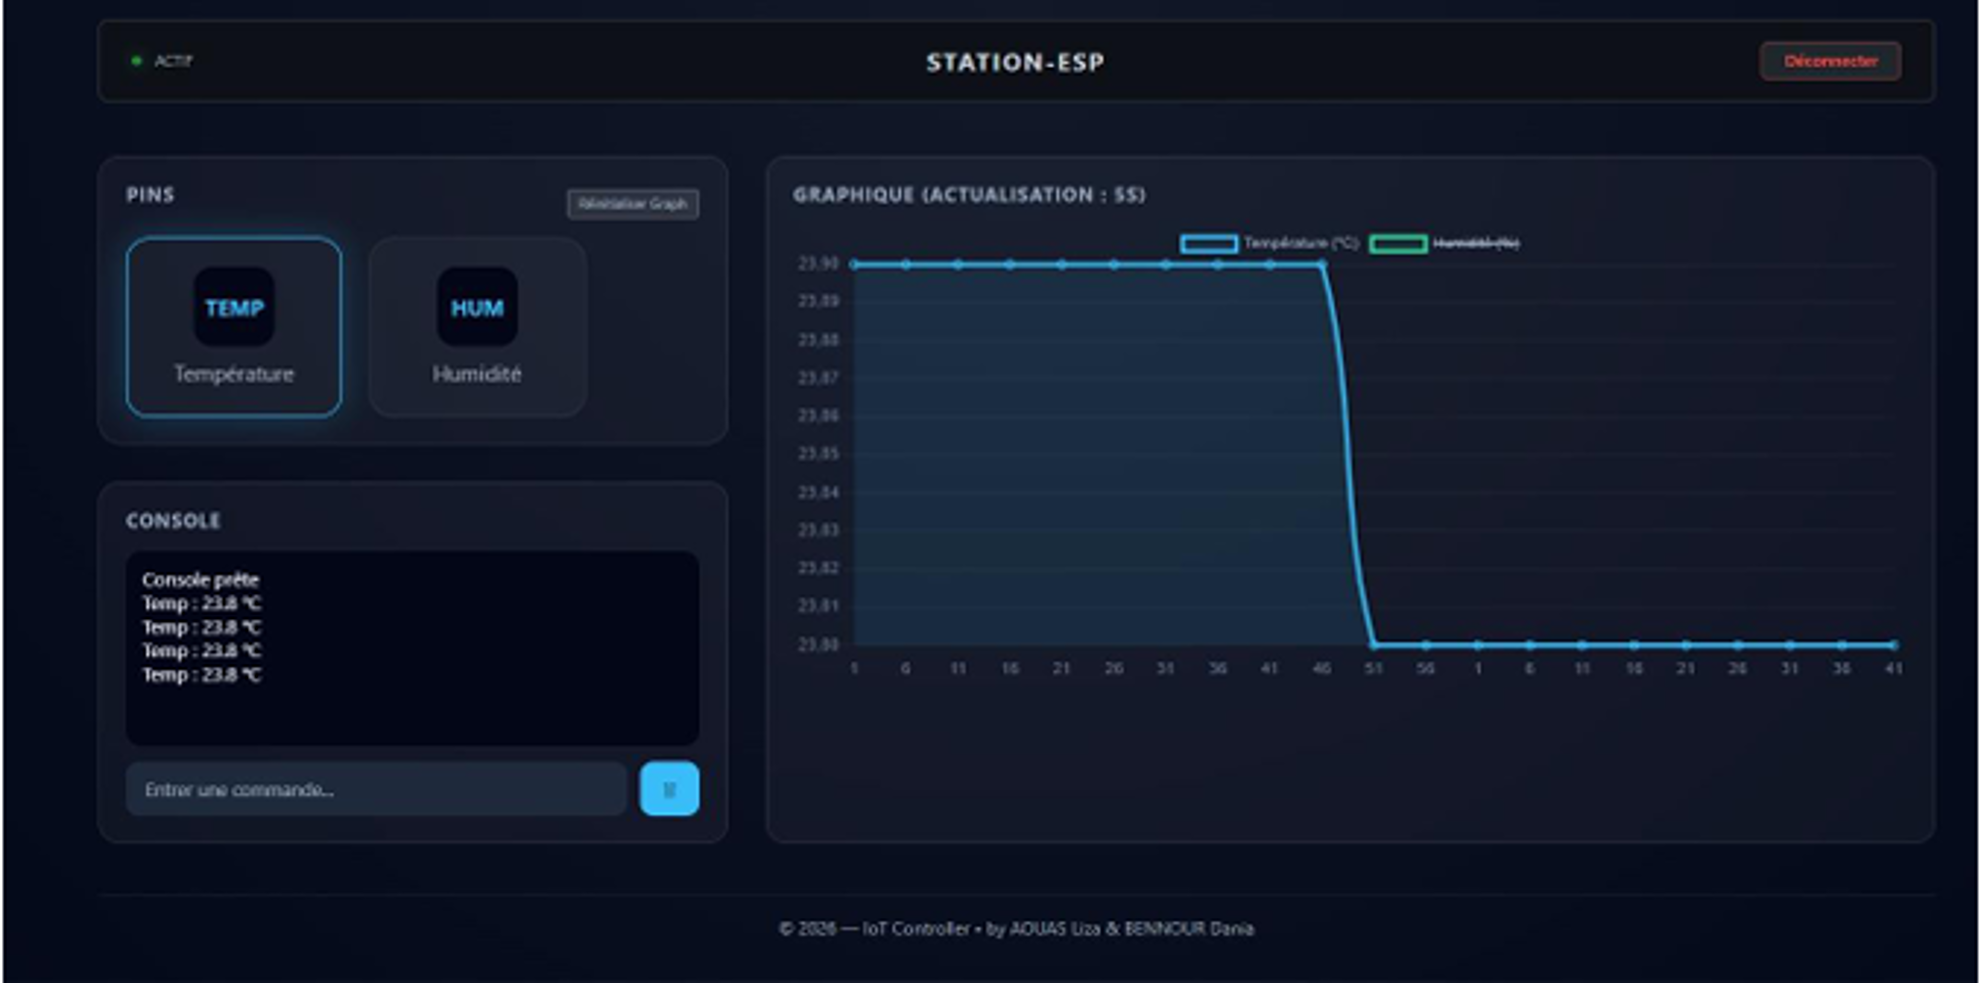
\includegraphics[width=\linewidth]{PictureS7.png}
  \caption{Interface du POC (Semestre 7)}
\end{minipage}
\hfill
\begin{minipage}[b]{0.48\textwidth}
  \centering
  
  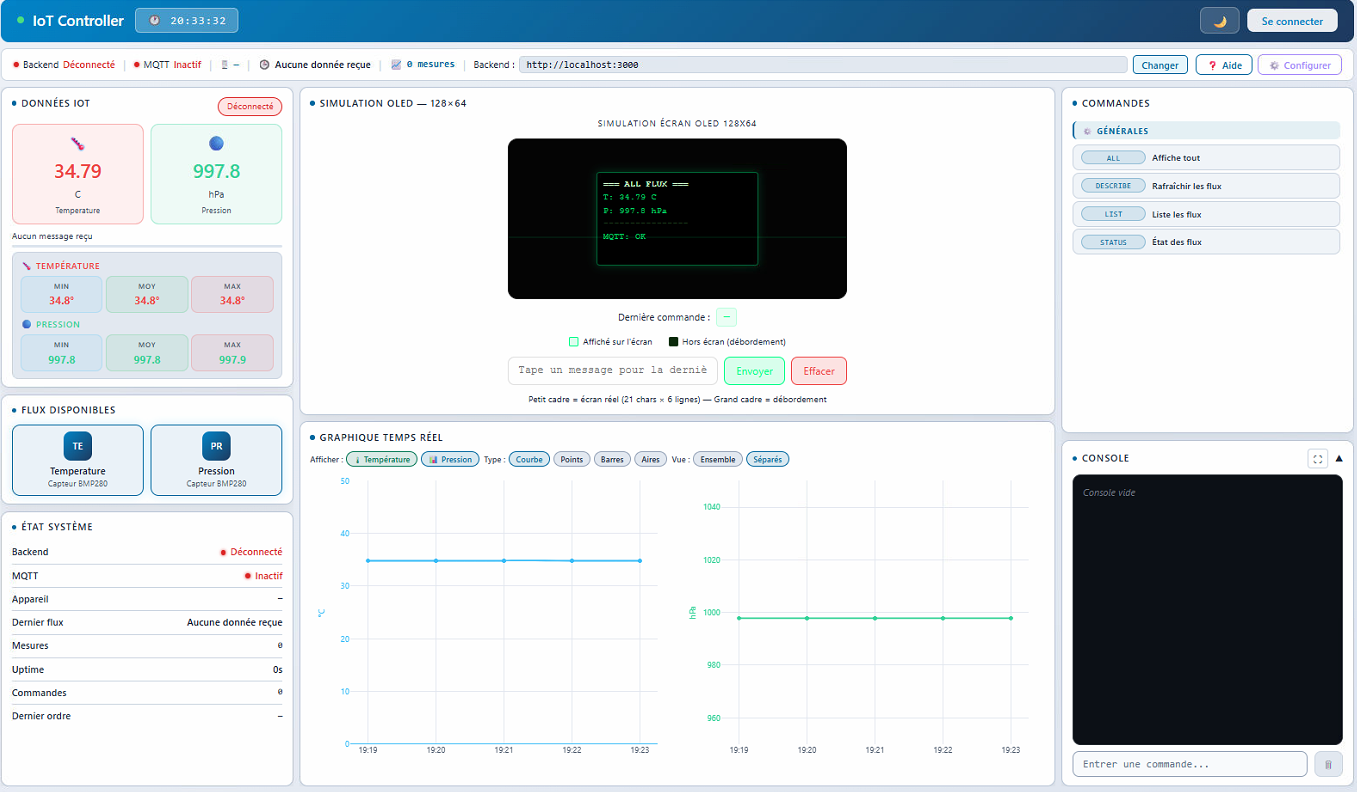
\includegraphics[width=\linewidth]{dashboard-S8.png}
  \caption{Nouveau Dashboard PWA (V1.0)}
\end{minipage}
\vspace{0.2cm}
\caption{Comparaison visuelle entre l'interface initiale et le dashboard distribu\'e}
\label{fig:avant_apres}
\end{figure}

\subsection{Gestion des donn\'ees en temps r\'eel}

Le tableau~\ref{tab:donnees} pr\'esente les fonctionnalit\'es de
gestion des donn\'ees du dashboard. La caract\'eristique principale
est son \textbf{interface universelle} : aucun capteur n'est cod\'e
en dur, l'interface se configure automatiquement \`a partir des
m\'etadonn\'ees JSON envoy\'ees par l'ESP8266.

\begin{table}[H]
\centering
\renewcommand{\arraystretch}{1.3}
\begin{tabularx}{\linewidth}{|l|X|}
\hline
\rowcolor{bleuFonce!10}
\textbf{Fonctionnalit\'e} & \textbf{Description} \\
\hline
Interface universelle &
  Aucun capteur cod\'e en dur -- pilot\'ee par m\'etadonn\'ees JSON \\
\hline
Auto-configuration &
  G\'en\'eration dynamique depuis \texttt{deviceId/metadata/flows} \\
\hline
Couleur temp\'erature &
  Bleu ($<20$\textdegree C) / Vert ($20-30$\textdegree C) /
  Rouge ($>30$\textdegree C) \\
\hline
Couleur pression &
  Orange ($<980$ hPa) / Vert ($980-1020$ hPa) / Bleu ($>1020$ hPa) \\
\hline
Badges Min/Moy/Max &
  Affichage color\'e avec \'evolutions graphiques \\
\hline
Barre de fra\^icheur &
  Barre horizontale : Verte $\to$ Orange $\to$ Rouge \\
\hline
Horodatage relatif &
  Affichage ``il y a X secondes/minutes/heures'' \\
\hline
Uptime depuis connexion &
  Compteur en direct depuis la connexion MQTT \\
\hline
Compteur commandes &
  Nombre de commandes envoy\'ees + dernier ordre \\
\hline
\end{tabularx}
\caption{Gestion des donn\'ees temps r\'eel du dashboard}
\label{tab:donnees}
\end{table}

\subsection{Graphique Plotly.js interactif}

\begin{infobox}[Pourquoi Plotly.js plut\^ot que Chart.js ?]
Plusieurs biblioth\`eques de graphiques JavaScript ont \'et\'e
\'evalu\'ees avant de retenir Plotly.js, notamment \textbf{Chart.js},
utilis\'ee dans de nombreux tutoriels IoT. Le choix final s'est port\'e
sur Plotly.js pour les raisons suivantes~:
\begin{itemize}[leftmargin=0.8cm, itemsep=3pt]
  \item[\ding{51}] \textbf{Interactions natives avanc\'ees~:} zoom,
        d\'ezoom et export PNG int\'egr\'es sans code suppl\'ementaire,
        l\`a o\`u Chart.js n\'ecessite des plugins tiers.
  \item[\ding{51}] \textbf{Richesse des types de trac\'e~:} 5 modes
        (courbe, points, barres, aires, ensemble) disponibles
        nativement avec la m\^eme API.
  \item[\ding{51}] \textbf{Performance sur s\'eries temporelles~:}
        gestion optimis\'ee des grands volumes de points, adapt\'ee
        \`a un flux de donn\'ees continu toutes les 5 secondes.
  \item[\ding{51}] \textbf{Origine scientifique~:} biblioth\`eque
        issue de l'\'ecosyst\`eme Python/R, r\'eput\'ee pour la
        pr\'ecision de ses axes et de son \'echelle temporelle,
        un atout pour un projet de mesure et traitement de
        l'information.
\end{itemize}
Chart.js reste plus l\'eger en taille de fichier, mais Plotly.js a
\'et\'e jug\'e plus adapt\'e \`a un dashboard de supervision
professionnelle n\'ecessitant des interactions riches.
\end{infobox}

Le tableau~\ref{tab:plotly} pr\'esente les caract\'eristiques du
graphique temps r\'eel. Plotly.js offre cinq types de trac\'e et des
interactions natives (zoom, d\'ezoom, export PNG), avec un historique
glissant des 50 derni\`eres mesures affich\'e en heures r\'eelles au
format HH:MM.

\begin{table}[H]
\centering
\renewcommand{\arraystretch}{1.3}
\begin{tabularx}{\linewidth}{|l|X|}
\hline
\rowcolor{bleuFonce!10}
\textbf{Fonctionnalit\'e} & \textbf{Description} \\
\hline
Axe X temps r\'eel &
  Heures r\'eelles au format HH:MM (ex: 14:32, 15:47) \\
\hline
5 types de trac\'e &
  Courbe liss\'ee / Points discrets / Barres / Aires / Ensemble \\
\hline
Vue s\'epar\'ee/ensemble &
  2 graphiques c\^ote \`a c\^ote ou 1 graphique fusion\'e \\
\hline
Historique 50 mesures &
  Fen\^etre glissante des 50 derniers points \\
\hline
Zoom et d\'ezoom & Interaction souris Plotly native \\
\hline
Export PNG & Bouton ``Save as PNG'' dans la barre Plotly \\
\hline
Lisibilit\'e axe X &
  Maximum 6 ticks pour \'eviter surcharge textuelle \\
\hline
\end{tabularx}
\caption{Caract\'eristiques du graphique Plotly.js}
\label{tab:plotly}
\end{table}

\subsection{Console de logs et commandes}

Le tableau~\ref{tab:console} pr\'esente les fonctionnalit\'es de la
console et du panneau de commandes. La console affiche les
\'ev\'enements syst\`eme en temps r\'eel avec un code couleur par
type de message, tandis que les boutons de commandes sont
\textbf{g\'en\'er\'es automatiquement} depuis les m\'etadonn\'ees de
l'ESP8266, sans aucun codage en dur.

\begin{table}[H]
\centering
\renewcommand{\arraystretch}{1.3}
\begin{tabularx}{\linewidth}{|l|X|}
\hline
\rowcolor{bleuFonce!10}
\textbf{Fonctionnalit\'e} & \textbf{Description} \\
\hline
Logs color\'es par type &
  Vert (OK) / Bleu (INFO) / Rouge (ERREUR) / Violet (WARN) /
  Jaune (\'EV\'ENEMENT) \\
\hline
Mode r\'etractable &
  Bouton $\blacktriangle$/$\blacktriangledown$ pour r\'eduire \\
\hline
Mode plein \'ecran & Overlay 85vw $\times$ 80vh avec fermeture \\
\hline
Bouton Effacer & Vide l'historique des logs affich\'es \\
\hline
Boutons auto-g\'en\'er\'es &
  Cr\'e\'es dynamiquement depuis les flux des m\'etadonn\'ees \\
\hline
Bouton actif persistant &
  Fond bleu plein pour indiquer la s\'election \\
\hline
Panneau Configurer &
  D\'epla\c{c}able, pour modifier les param\`etres backend \\
\hline
Panneau Aide &
  D\'epla\c{c}able avec recherche filtrante des 9 commandes \\
\hline
Multi-clients valid\'e &
  2+ navigateurs re\c{c}oivent les m\^emes donn\'ees instantan\'ement \\
\hline
\end{tabularx}
\caption{Fonctionnalit\'es console, commandes et aide contextuelle}
\label{tab:console}
\end{table}

\section{Architecture des composants Vue.js 3}

La figure~\ref{fig:composants} illustre l'arborescence des composants
Vue.js 3 du dashboard. Le composant \texttt{Dashboard.vue} joue le
r\^ole d'\textbf{orchestrateur principal} : il re\c{c}oit les donn\'ees
du backend via Socket.IO et les distribue aux composants enfants,
chacun responsable d'une fonctionnalit\'e pr\'ecise de l'interface.

\begin{figure}[H]
\centering
\resizebox{\linewidth}{!}{%
\begin{tikzpicture}[
  main/.style={rectangle, rounded corners=5pt, draw=bleuFonce,
    fill=bleuFonce!10, thick, minimum width=5.0cm,
    minimum height=1.1cm, align=center, font=\small\bfseries},
  comp/.style={rectangle, rounded corners=4pt, draw=bleuPrincipal,
    fill=bleuClair, thick, minimum width=3.0cm,
    minimum height=1.0cm, align=center, font=\scriptsize},
  arr/.style={-{Stealth[length=2.5mm, width=1.8mm]}, thick,
    draw=bleuPrincipal},
]
\node[main] (dash) at (0, 0)
  {\textcolor{bleuFonce}{Dashboard.vue}\\[2pt]
   {\scriptsize Composant Orchestrateur Principal}};
\node[comp] (chart)   at (-7.0, -2.8)
  {ChartPanel.vue\\[2pt]{\tiny Graphique Plotly.js}};
\node[comp] (oled)    at (-2.5, -2.8)
  {OledScreen.vue\\[2pt]{\tiny Simulateur OLED}};
\node[comp] (console) at ( 2.5, -2.8)
  {ConsolePanel.vue\\[2pt]{\tiny Console logs}};
\node[comp] (config)  at ( 7.0, -2.8)
  {CommandConfig.vue\\[2pt]{\tiny Configuration}};
\node[comp] (help)    at (-2.5, -5.2)
  {HelpPanel.vue\\[2pt]{\tiny Aide contextuelle}};
\node[comp] (footer)  at ( 2.5, -5.2)
  {FooterBar.vue\\[2pt]{\tiny Pied de page}};
\foreach \c in {chart, oled, console, config, help, footer}
  \draw[arr] (dash) -- (\c);
\end{tikzpicture}
}
\caption{Arborescence des composants Vue.js 3 de l'architecture
         distribu\'ee}
\label{fig:composants}
\end{figure}

\section{M\'ecanisme d'\'ecoute g\'en\'erique et universelle}

Le listing~\ref{lst:ecoute} pr\'esente le m\'ecanisme central de
l'interface universelle. Gr\^ace \`a \texttt{socket.onAny()}, le
dashboard \'ecoute \textbf{tous les flux IoT dynamiquement} sans
aucun capteur cod\'e en dur. Chaque nouveau flux d\'etect\'e est
automatiquement stock\'e dans une Map g\'en\'erique et affich\'e
dans l'interface. C'est ce m\'ecanisme qui rend le syst\`eme
adaptable \`a n'importe quel dispositif IoT sans modifier une seule
ligne de code du dashboard.

\begin{lstlisting}[caption={\'Ecoute universelle de tous les flux IoT
                   via socket.onAny()}, label={lst:ecoute}]
// Interface universelle : ecouter TOUS les evenements
socket.on('flux-metadata', (data) => {
  deviceId.value     = data.id;
  fluxMetadata.value = data.flows;
  // L'interface se configure automatiquement
});

// Ecoute generique de tous les flux
socket.onAny((eventName, data) => {
  if (!eventName.endsWith('-data')) return;
  const fluxId = eventName.replace('-data', '');

  // Stockage generique -- aucun capteur code en dur
  fluxValues.value[fluxId]     = data.value;
  fluxUnits.value[fluxId]      = data.unit;
  fluxTimestamps.value[fluxId] = new Date();

  // Mise a jour graphiques Plotly dynamiques
  updatePlotlyChart(fluxId, data.value);
});
\end{lstlisting}

% ==========================================
% CHAPITRE 7 -- Tests
% ==========================================
\chapter{Tests et validation}

\section{Campagne de tests fonctionnels}

Le tableau~\ref{tab:tests} pr\'esente les r\'esultats de la campagne
de tests fonctionnels r\'ealis\'ee sur l'ensemble du syst\`eme. Les
onze sc\'enarios test\'es couvrent la cha\^ine compl\`ete, de la
r\'eception des donn\'ees MQTT jusqu'\`a l'installation PWA, et ont
tous \'et\'e valid\'es avec succ\`es.

\begin{table}[H]
\centering
\renewcommand{\arraystretch}{1.35}
\begin{tabularx}{\linewidth}{|l|X|c|}
\hline
\rowcolor{bleuFonce!10}
\textbf{Sc\'enario} & \textbf{Description} & \textbf{R\'esultat} \\
\hline
R\'eception donn\'ees MQTT &
  BMP280 publie toutes les 5 secondes &
  \textcolor{vertOK}{\ding{51} OK} \\
\hline
M\'etadonn\'ees RETAIN &
  Backend d\'emarre apr\`es l'Arduino &
  \textcolor{vertOK}{\ding{51} OK} \\
\hline
2 navigateurs simultan\'es &
  M\^emes donn\'ees au m\^eme instant &
  \textcolor{vertOK}{\ding{51} OK} \\
\hline
9 commandes MQTT &
  ALL, TEMP, PRESS, LIST, STATUS, DESCRIBE, etc. &
  \textcolor{vertOK}{\ding{51} OK} \\
\hline
OLED physique r\'eagit &
  \'Ecran affiche les r\'esultats de chaque commande &
  \textcolor{vertOK}{\ding{51} OK} \\
\hline
Mode hors-ligne &
  Bandeau rouge, donn\'ees conserv\'ees en cache &
  \textcolor{vertOK}{\ding{51} OK} \\
\hline
Reconnexion automatique &
  R\'etablissement apr\`es coupure Wi-Fi &
  \textcolor{vertOK}{\ding{51} OK} \\
\hline
Th\`eme clair/sombre &
  Toggle et persistance localStorage &
  \textcolor{vertOK}{\ding{51} OK} \\
\hline
Console plein \'ecran &
  Overlay 85vw $\times$ 80vh &
  \textcolor{vertOK}{\ding{51} OK} \\
\hline
Uptime et horodatage &
  Compteurs synchronis\'es &
  \textcolor{vertOK}{\ding{51} OK} \\
\hline
PWA installation &
  Ic\^one bureau, mode app native &
  \textcolor{vertOK}{\ding{51} OK} \\
\hline
\end{tabularx}
\caption{R\'esultats de la campagne de tests fonctionnels}
\label{tab:tests}
\end{table}

\section{Probl\`emes r\'esolus pendant le d\'eveloppement}

Le tableau~\ref{tab:problemes} recense les principaux probl\`emes
rencontr\'es durant le d\'eveloppement et leurs solutions. Ces
obstacles, li\'es aux contraintes m\'emoire de l'ESP8266, au protocole
MQTT et \`a l'affichage, ont tous \'et\'e r\'esolus et ont contribu\'e
\`a renforcer la robustesse et la fiabilit\'e du syst\`eme final.

\begin{table}[H]
\centering
\renewcommand{\arraystretch}{1.4}
\begin{tabularx}{\linewidth}{|l|X|X|}
\hline
\rowcolor{bleuFonce!10}
\textbf{Probl\`eme} & \textbf{Cause} & \textbf{Solution} \\
\hline
Crash ESP8266 (out of memory) &
  \texttt{setBufferSize(512)} d\'epassait la m\'emoire &
  Suppression du buffer, payloads $<140$ octets \\
\hline
Refus connexion HiveMQ &
  ClientId dupliqu\'e entre sessions &
  G\'en\'eration clientId al\'eatoire \`a chaque d\'emarrage \\
\hline
OLED noir sur PRESSION &
  Mapping topic manquant (casse) &
  Mapping explicite : \texttt{PRESSION} $\to$ \texttt{PRESS} \\
\hline
Axe X Plotly illisible &
  Trop d'\'etiquettes HH:MM &
  Limitation \`a max 6 ticks \\
\hline
Wildcard MQTT refus\'e &
  Pattern \texttt{+/+/+} trop g\'en\'erique &
  Utilisation \texttt{+/datalog/+/+} (4 blocs) \\
\hline
M\'etadonn\'ees manquantes &
  Backend d\'emarr\'e avant l'Arduino &
  Flag RETAIN + commande DESCRIBE automatique \\
\hline
\end{tabularx}
\caption{Probl\`emes r\'esolus durant le d\'eveloppement et d\'eploiement}
\label{tab:problemes}
\end{table}

\section{M\'etriques de performance et dimensionnement}

Le tableau~\ref{tab:performance} pr\'esente les indicateurs de
performance mesur\'es sur le syst\`eme complet. Le r\'esultat le plus
significatif est le d\'elai bout en bout inf\'erieur \`a
\textbf{100 ms}, du capteur BMP280 jusqu'au navigateur, avec seulement
37\,\% de la RAM de l'ESP8266 utilis\'ee, confirmant la l\'eg\`eret\'e
et l'efficacit\'e de l'architecture choisie.

\begin{table}[H]
\centering
\renewcommand{\arraystretch}{1.3}
\begin{tabular}{|l|c|}
\hline
\rowcolor{bleuFonce!10}
\textbf{M\'etrique} & \textbf{Valeur} \\
\hline
Fr\'equence publication MQTT & 1 mesure / 5 secondes \\
\hline
D\'elai bout en bout (capteur $\to$ navigateur) & $< 100$ ms \\
\hline
Taille payload JSON par mesure & $\approx 38$ octets \\
\hline
RAM ESP8266 utilis\'ee & 37\,\% (30\,352 / 80\,192 octets) \\
\hline
Flash ESP8266 utilis\'e & 26\,\% (275\,520 / 1\,048\,576 octets) \\
\hline
Historique graphique & 50 derni\`eres mesures \\
\hline
Nombre de commandes impl\'ement\'ees & 9 commandes MQTT \\
\hline
Clients simultan\'es test\'es & 2+ avec succ\`es \\
\hline
\end{tabular}
\caption{Indicateurs de performance du syst\`eme distribu\'e}
\label{tab:performance}
\end{table}

% ==========================================
% CHAPITRE 8 -- Conclusion
% ==========================================
\chapter{Conclusion g\'en\'erale et perspectives}

\section{Bilan du d\'eploiement final}

Ce projet a permis de transformer une application de base (POC) en
une \textbf{plateforme de supervision IoT professionnelle, universelle
et modulable}. Les \'evolutions apport\'ees r\'epondent directement
\`a chacune des limites initiales~:

\begin{itemize}[leftmargin=1.5cm, itemsep=5pt]
  \item La \textbf{d\'ependance au c\^able USB} a \'et\'e enti\`erement
        \'elimin\'ee gr\^ace \`a MQTT et au Wi-Fi embarqu\'e.
  \item L'\textbf{interface fig\'ee} a \'et\'e remplac\'ee par une
        architecture universelle pilot\'ee par m\'etadonn\'ees JSON.
  \item Les \textbf{2 commandes rudimentaires} sont devenues
        \textbf{9 commandes riches et contextuelles}.
  \item L'\textbf{absence d'affichage local} a \'et\'e combl\'ee avec
        un \'ecran OLED physique synchronis\'e.
  \item Le \textbf{manque de port\'ee} a \'et\'e r\'esolu~:
        supervision Wi-Fi sur r\'eseau entier.
  \item Le \textbf{mode hors-ligne et la PWA} ont \'et\'e enti\`erement
        impl\'ement\'es.
  \item Le \textbf{support multi-clients} valide les d\'eploiements
        d'\'equipe.
\end{itemize}

\section{Atteinte des objectifs}

\begin{successbox}[R\'ecapitulatif des objectifs r\'ealis\'es]
\begin{itemize}[leftmargin=1cm, itemsep=4pt]
  \item[\ding{51}] MQTT remplace la liaison s\'erie --
        communication sans fil standardis\'ee
  \item[\ding{51}] ESP8266 communique de fa\c{c}on autonome via Wi-Fi
  \item[\ding{51}] BMP280 remplace DHT11 --
        capteur plus pr\'ecis avec pression
  \item[\ding{51}] OLED SSD1306 int\'egr\'e --
        affichage local synchronis\'e
  \item[\ding{51}] Interface universelle --
        \textbf{0 ligne de code} \`a modifier pour ajouter un capteur
  \item[\ding{51}] Dashboard professionnel avec Plotly.js (5 trac\'es)
        et PWA
  \item[\ding{51}] Communication bidirectionnelle --
        9 commandes downlink vers Arduino
\end{itemize}
\end{successbox}

\section{Analyse critique du projet}

Si je devais recommencer ce projet, trois choix techniques seraient
revus~:

\begin{itemize}[leftmargin=1.5cm, itemsep=6pt]
  \item \textbf{Broker MQTT public HiveMQ~:} L'utilisation d'un
        broker public pr\'esente des risques de s\'ecurit\'e et de
        disponibilit\'e, le service \'etant partag\'e avec des
        milliers d'autres utilisateurs anonymes. Un broker priv\'e
        (Mosquitto en local ou CloudMQTT) aurait \'et\'e plus robuste
        pour un d\'eploiement industriel r\'eel.
  \item \textbf{Absence de base de donn\'ees~:} L'historique des
        mesures est limit\'e \`a 50 points conserv\'es en m\'emoire
        vive c\^ot\'e navigateur. Int\'egrer une base de donn\'ees
        temporelle comme InfluxDB d\`es la conception aurait permis
        une analyse long terme des donn\'ees et la persistance entre
        les sessions.
  \item \textbf{Absence d'authentification~:} Le dashboard est
        accessible sans mot de passe \`a quiconque conna\^it
        l'adresse r\'eseau. Dans un contexte industriel r\'eel, une
        authentification (JWT ou OAuth) aurait \'et\'e indispensable
        avant tout d\'eploiement en production.
\end{itemize}

Ces trois limites identifi\'ees constituent pr\'ecis\'ement les axes
prioritaires des perspectives d'\'evolution d\'ecrites ci-apr\`es.

\section{Perspectives d'\'evolution future}

\begin{itemize}[leftmargin=1.5cm, itemsep=6pt]
  \item \textbf{Persistance des donn\'ees :} Int\'egrer InfluxDB ou
        Firebase pour conserver l'historique au-del\`a de 50 points.
  \item \textbf{Multi-appareils :} G\'erer plusieurs ESP8266
        simultan\'ement avec s\'electeur de device.
  \item \textbf{Alertes automatiques :} Notifications (email, SMS,
        Web Push) quand une valeur d\'epasse un seuil configurable.
  \item \textbf{S\'ecurisation MQTTS :} Chiffrer les communications
        avec TLS/SSL.
  \item \textbf{D\'eploiement cloud :} H\'eberger le backend Node.js
        sur AWS, Azure ou Heroku.
  \item \textbf{Authentification utilisateur :} Login/register avec
        JWT pour acc\`es s\'ecuris\'e.
  \item \textbf{Tableau de bord personnalis\'e :} Drag-and-drop des
        widgets pour organisation libre.
\end{itemize}

\section{R\'eflexions finales}

Ce projet d\'emontre la valeur d'une approche it\'erative et extensible
dans le d\'eveloppement IoT. En privil\'egiant une architecture
loosely-coupled (MQTT), universellement configurable (m\'etadonn\'ees),
et r\'esiliente (PWA + offline-first), j'ai cr\'e\'e une fondation
robuste pour des d\'eploiements futurs.

L'interface enti\`erement g\'en\'er\'ee par m\'etadonn\'ees est le
v\'eritable pivot de cette r\'eussite~: elle rend le syst\`eme
adaptable \`a d'autres capteurs, d'autres d\'ebits, d'autres
topologies, sans une seule ligne de code \`a modifier. C'est
pr\'ecis\'ement cette caract\'eristique qui diff\'erencie ce projet
d'une simple console IoT et en fait une \textbf{plateforme de
supervision g\'en\'erique} r\'eutilisable dans tout contexte industriel.

Sur le plan personnel, ce projet m'a permis de ma\^itriser une cha\^ine
technologique compl\`ete et repr\'esentative de l'IoT industriel~: du
firmware embarqu\'e jusqu'\`a l'interface utilisateur, en passant par
les protocoles de communication et le d\'eveloppement backend. La
gestion en solo de l'ensemble de la stack technique, de la conception
\`a la documentation, a consid\'erablement renforc\'e mon autonomie et
ma rigueur d'ing\'enieure.

% ==========================================
% ANNEXES
% ==========================================
\appendix

\chapter{Rappel de la preuve de concept (POC)}

\section{Composants et architecture du POC}

Le tableau~\ref{tab:poc} rappelle l'architecture du projet r\'ealis\'e
au Semestre~7 en bin\^ome. Ce POC, bas\'e sur une communication s\'erie
USB, constituait une premi\`ere approche locale et limit\'ee, sans
protocole IoT standard, sans mode hors-ligne et sans support
multi-clients, lacunes que le projet Semestre~8 vient directement
combler.

\begin{table}[H]
\centering
\renewcommand{\arraystretch}{1.4}
\begin{tabularx}{\linewidth}{|l|X|}
\hline
\rowcolor{bleuFonce!10}
\textbf{Composant POC} & \textbf{Description} \\
\hline
ESP8266 + DHT11 &
  Lecture temp\'erature et humidit\'e, envoi via port s\'erie USB
  \`a 9600 baud \\
\hline
Node.js + SerialPort &
  \'Ecoute du port COM, redistribution via Socket.IO aux clients \\
\hline
Vue.js (simple) &
  Interface basique : console s\'erie, graphique simple, boutons
  START/STOP \\
\hline
Commandes &
  START (d\'emarrer la lecture) et STOP (arr\^eter la lecture) \\
\hline
Mode offline & Non disponible \\
\hline
Multi-clients & Non support\'e \\
\hline
\end{tabularx}
\caption{Rappel de l'architecture du POC (Semestre 7)}
\label{tab:poc}
\end{table}

\chapter{Structure compl\`ete de l'architecture distribu\'ee}

Le listing~\ref{lst:arborescence} pr\'esente l'arborescence compl\`ete
des fichiers du projet. Le code est organis\'e en trois dossiers
principaux : \texttt{backend/} pour le serveur Node.js,
\texttt{frontend/} pour le dashboard Vue.js et ses composants, et
\texttt{arduino\_export/} pour le firmware ESP8266.

\begin{lstlisting}[caption={Arborescence des fichiers du projet final},
                  label={lst:arborescence}]
MON_PROJETS8/
|
|-- backend/
|   |-- server.js         # Point d'entree -- MQTT + Socket.IO
|   |-- .env              # Variables d'environnement
|   |-- package.json      # Dependances Node.js
|   `-- .gitignore
|
|-- frontend/
|   |-- src/
|   |   |-- views/
|   |   |   `-- Dashboard.vue       # Composant orchestrateur
|   |   |-- components/
|   |   |   |-- ChartPanel.vue      # Graphique Plotly.js
|   |   |   |-- ConsolePanel.vue    # Console de logs
|   |   |   |-- OledScreen.vue      # Simulateur OLED virtuel
|   |   |   |-- CommandConfig.vue   # Configuration commandes
|   |   |   |-- HelpPanel.vue       # Aide contextuelle
|   |   |   `-- FooterBar.vue       # Pied de page
|   |   |-- assets/
|   |   |   `-- style.css           # Variables CSS themes
|   |   `-- main.js                 # Point d'entree Vue 3
|   |-- vite.config.js              # Configuration Vite + PWA
|   |-- package.json
|   `-- index.html
|
`-- arduino_export/
    `-- arduino_code.ino            # Firmware ESP8266 complet
\end{lstlisting}

\chapter{Guide de d\'emarrage du projet}

\section{Variables d'environnement backend (\texttt{.env})}

Le listing~\ref{lst:env} pr\'esente le fichier de configuration
\texttt{.env} du backend. Il centralise les param\`etres essentiels du
syst\`eme, permettant de modifier la configuration sans toucher au code
source.

\begin{lstlisting}[caption={Fichier .env du backend Node.js},
                  label={lst:env}]
PORT=3000
MQTT_BROKER=mqtt://broker.hivemq.com
SERIAL_PORT=COM3
SERIAL_BAUD=9600
NODE_ENV=development
\end{lstlisting}

\section{\'Etapes de d\'emarrage}

Le listing~\ref{lst:demarrage} pr\'esente la s\'equence compl\`ete de
lancement du syst\`eme en 5 \'etapes ordonn\'ees.
\textbf{L'ordre de ces \'etapes est imp\'eratif} pour \'eviter les
conflits de port s\'erie et garantir la bonne initialisation des
connexions MQTT et WebSocket.

\begin{lstlisting}[caption={S\'equence de lancement compl\`ete},
                  label={lst:demarrage}]
# 1. Fermer Arduino IDE (liberer le port COM3)

# 2. Demarrer le backend Node.js
cd MON_PROJETS8/backend
npm install
node server.js
# Serveur demarre sur http://localhost:3000

# 3. Demarrer le frontend (nouveau terminal)
cd MON_PROJETS8/frontend
npm install
serve -s dist -l 4173
# Acces sur http://localhost:4173

# 4. Flash du firmware Arduino
# Ouvrir arduino_export/arduino_code.ino
# Modifier : const char* ssid = "MON_WIFI";
#            const char* password = "MON_PASS";
# Carte : NodeMCU 1.0 (ESP-12E Module)
# Uploader (Ctrl+U)

# 5. Ouvrir le navigateur
# http://localhost:4173
\end{lstlisting}

\section{V\'erification du d\'eploiement}

\begin{successbox}[Checklist de validation]
\begin{itemize}[leftmargin=0.8cm, itemsep=3pt]
  \item[\ding{51}] Backend Node.js sur localhost:3000
  \item[\ding{51}] Frontend sur localhost:4173
  \item[\ding{51}] ESP8266 flash\'e et connect\'e au Wi-Fi
  \item[\ding{51}] Donn\'ees apparaissent dans le dashboard
  \item[\ding{51}] Graphique Plotly mis \`a jour toutes les 5s
  \item[\ding{51}] OLED physique affiche les valeurs
  \item[\ding{51}] Les 9 commandes r\'epondent correctement
  \item[\ding{51}] Mode hors-ligne fonctionne
  \item[\ding{51}] PWA peut \^etre install\'ee
\end{itemize}
\end{successbox}

\chapter{Manuel d'Installation}

Cliquez sur le bouton ci-dessous pour ouvrir le Manuel d'Installation
complet~:

\vspace{1cm}
\begin{center}
\begin{tcolorbox}[
  enhanced, colback=bleuClair, colframe=bleuPrincipal,
  boxrule=1.5pt, arc=6pt, width=0.72\textwidth,
  halign=center, left=12pt, right=12pt,
  top=14pt, bottom=14pt,
]
  \href{https://drive.google.com/file/d/1IoyHiOMMlWHxrSSMEAeaRcc7evhafhab/view?usp=drive_link}{%
    \textcolor{bleuFonce}{\Large\bfseries
    $\triangleright$\enspace Ouvrir le Manuel d'Installation}%
  }\\[8pt]
  {\small\textcolor{griMoyen}{Disponible sur Google Drive}}
\end{tcolorbox}
\end{center}

\chapter{Manuel d'Utilisation}

Cliquez sur le bouton ci-dessous pour ouvrir le Manuel d'Utilisation
complet~:

\vspace{1cm}
\begin{center}
\begin{tcolorbox}[
  enhanced, colback=bleuClair, colframe=bleuPrincipal,
  boxrule=1.5pt, arc=6pt, width=0.72\textwidth,
  halign=center, left=12pt, right=12pt,
  top=14pt, bottom=14pt,
]
  \href{https://drive.google.com/file/d/1Pbwp4Xd4XEElCwQaQ0MdwwGoU7PmZTh9/view?usp=drive_link}{%
    \textcolor{bleuFonce}{\Large\bfseries
    $\triangleright$\enspace Ouvrir le Manuel d'Utilisation}%
  }\\[8pt]
  {\small\textcolor{griMoyen}{Disponible sur Google Drive}}
\end{tcolorbox}
\end{center}

\chapter{Vid\'eo de d\'emonstration}

Cliquez sur le bouton ci-dessous pour visionner la d\'emonstration
compl\`ete de l'application IoT Controller, pr\'esentant l'interface,
l'envoi de commandes, le simulateur OLED et la g\'en\'eration
automatique de l'interface depuis les m\'etadonn\'ees~:

\vspace{1cm}
\begin{center}
\begin{tcolorbox}[
  enhanced, colback=bleuClair, colframe=bleuPrincipal,
  boxrule=1.5pt, arc=6pt, width=0.72\textwidth,
  halign=center, left=12pt, right=12pt,
  top=14pt, bottom=14pt,
]
  \href{https://drive.google.com/file/d/1ZKkiPMIA36Nbi1gCWcmVh21lzbyH2on8/view?usp=sharing}{%
    \textcolor{bleuFonce}{\Large\bfseries
    $\triangleright$\enspace Visionner la d\'emonstration vid\'eo}%
  }\\[8pt]
  {\small\textcolor{griMoyen}{Disponible sur Google Drive}}
\end{tcolorbox}
\end{center}

\chapter{Bibliographie et ressources}

\section{Documentation officielle}

\begin{itemize}[leftmargin=1.5cm, itemsep=5pt]
  \item Vue.js 3 Composition API :
        \url{https://vuejs.org/guide/extras/composition-api-faq.html}
  \item Sp\'ecification MQTT 3.1.1 :
        \url{https://mqtt.org/mqtt-specification}
  \item Socket.IO Documentation :
        \url{https://socket.io/docs/}
  \item Plotly.js API Reference :
        \url{https://plotly.com/javascript/}
  \item PubSubClient Arduino :
        \url{https://pubsubclient.knolleary.net/}
  \item Adafruit BMP280 Library :
        \url{https://github.com/adafruit/Adafruit_BMP280_Library}
  \item Adafruit SSD1306 Library :
        \url{https://github.com/adafruit/Adafruit_SSD1306}
  \item HiveMQ Public Broker :
        \url{https://www.hivemq.com/public-mqtt-broker/}
  \item Vite PWA Plugin :
        \url{https://vite-pwa-org.netlify.app/}
\end{itemize}

\section{R\'ef\'erences technologiques}

\begin{itemize}[leftmargin=1.5cm, itemsep=5pt]
  \item ESP8266 Community Edition : Docs officiel firmware Arduino
  \item I2C Protocol : Standard multi-device sur 2 lignes (SDA/SCL)
  \item JSON Schema : D\'efinition et validation des structures de donn\'ees
  \item Progressive Web Apps (PWA) : D\'eveloppement d'applications Web
        natives
\end{itemize}

\section{R\'ef\'erences acad\'emiques et industrielles}

\begin{itemize}[leftmargin=1.5cm, itemsep=5pt]
  \item \textbf{Stanford-Clark, A., Nipper, A.} (1999).
        \textit{MQTT v3.1 Protocol Specification}.
        IBM developerWorks.
  \item \textbf{Placona, M., Fremantle, P.} (2016).
        \textit{MQTT and CoAP, IoT Protocols}.
        Eclipse Foundation White Paper.
  \item \textbf{Russell, A. et al.} (2015).
        \textit{Progressive Web Apps -- What, Why and How}.
        Google Developers.
  \item \textbf{You, E.} (2020).
        \textit{Vue 3 -- One Piece}.
        VueConf 2020, documentation officielle.
  \item \textbf{OASIS Standard} (2019).
        \textit{MQTT Version 5.0}.
        \url{https://docs.oasis-open.org/mqtt/mqtt/v5.0/}
\end{itemize}

\section{Accès au dépôt de code source (Annexe)}
\begin{itemize}[leftmargin=1.5cm, itemsep=5pt]
Le code source complet du projet, incluant le firmware, le backend Node.js et l'application PWA, est accessible via le dépôt GitHub suivant ainsi le code de rapport et des manuels d'utilisation et installation en latex:
\\
\fbox{\url{https://github.com/Liza2473/mon_projets8}}
\end{itemize}

\end{document}